\graphicspath{{./figures/5-hyperblock-scheduling/}}

\chapter{Verified Hyperblock Scheduling}%
\label{sec:hyperblock-scheduling}

\begin{chapsummary}
  This chapter describes the hyperblock scheduling pass in Vericert, which
  collects operations into groups that can be executed in parallel.  This
  chapter is based on a paper coauthored with John Wickerson which has been
  submitted to PLDI 2024 \cite[]{herklotz24_hsvhls}.
\end{chapsummary}

\noindent Many approaches to scheduling have been proposed over the years. Some, such as
\emph{\gls{list scheduling}}~\cite[][p.~257]{baker19_princ} only reorder instructions
within a basic block. This means they squander opportunities for performance
improvements that could be obtained by reordering instructions across
branches. A more powerful alternative is \emph{trace
  scheduling}~\cite{ellis85_bulld, fisher81_trace_sched}, which works by
creating paths (or `traces') through the code, across basic block boundaries,
and then reorders the instructions within those paths. In its most general
form, trace scheduling is considered infeasible on large programs, but two
special cases called \emph{superblock scheduling}~\cite{hwu93_super} and
\emph{hyperblock
  scheduling}~\cite{mahlke92_effec_compil_suppor_predic_execut_using_hyper} have
been developed, both of which impose restrictions on the form of traces in order
to obtain tractable algorithms. Superblocks generalise basic blocks by allowing
early exits, while hyperblocks generalise superblocks by additionally allowing each instruction to be \emph{predicated}. CPUs often lack support for predicated execution, so superblock scheduling is the natural choice in that setting.
But in custom hardware, predicated execution can be implemented efficiently, making hyperblock scheduling a natural fit for HLS.
Indeed, the use of
hyperblock scheduling in HLS was first proposed over two decades
ago~\cite{budiu02_compil_applic_specif_hardw,
  callahan98_instr_level_paral_recon_comput}, and is nowadays used by popular
HLS tools such as AMD Vitis
HLS~\cite{amd23_vitis_forum},  LegUp~\cite[][p.~60]{canis15_legup}, Google XLS~\cite[line~112]{google23_xls_uses_smt}, and Bambu~\cite[line~304]{ferrandi14_panda_bambu}.
Hyperblock scheduling is therefore a natural choice for Vericert to close the gap between the verified and unverified HLS tools, and model what existing tools are already doing.  Support for the scheduling of predicated instructions is also important for future HLS-specific optimisations, such as loop scheduling, because these often assume that basic blocks can be merged using if-conversion.

In this chapter, I present:

\begin{itemize}
\item \textbf{the first verified implementation of hyperblock scheduling}, which
  is more general than \citeauthor{six22_formal_verif_super_sched}'s verified
  superblock scheduler~\cite{six22_formal_verif_super_sched} and more
  computationally tractable than
  \citeauthor{tristan08_formal_verif_trans_valid}'s verified trace
  scheduler~\cite{tristan08_formal_verif_trans_valid},
\item \textbf{the first verified implementation of general if-conversion} (a
  pre-scheduling pass that turns if-statements into hyperblocks), building on
  CompCert's na\"ive if-converter that only handles simple
  cases~\cite{absint19_compc}, and
\item \textbf{a novel use of a verified SAT solver during translation
    validation} in order to reason about predicates.
\end{itemize}

First, \cref{sec:hs:overview} gives an overview of the scheduling optimisation,
then \cref{sec:hs:rtlblockdef} introduces the new intermediate languages used
for the scheduling transformation.  \Cref{sec:hs:if-conversion} then describes
hyperblock construction using if-conversion followed by
\cref{sec:hs:implementing-scheduling,sec:hs:verifying-scheduling,sec:hs:overview-validator-correctness-proof}
describing the implementation, validation and verification of the actual
hyperblock transformation.  Finally,
\cref{sec:hs:efficient-smt-solver-validation} describes the use of a validated
SMT solver as part of the hyperblock scheduling correctness proof.

\section{Overview}
\label{sec:hs:overview}

Making hardware designs parallel is actually not the challenging part of our work -- Verilog synthesis tools do this implicitly. Indeed, it is easy to write Verilog so that an arbitrary sequence of C operations is mapped to a single piece of combinational logic that executes in just one clock cycle. But the problem with such unfettered parallelism is that these large pieces of combinational logic may have long critical paths, and thus lead to hardware that can only run at a low clock frequency. The actual challenge, then, is producing the \emph{right amount} of parallelism.

This is a scheduling problem. Vericert must decide how to schedule each block of instructions across one or more clock cycles so that when the downstream Verilog synthesis tool performs parallelisation, the resulting combinational paths will be short enough to meet the target frequency.

To clarify: the downstream synthesis tool is responsible for the parallelisation itself -- Vericert does not perform it, nor does it guarantee its soundness. Rather, it predicts the parallelisation that the synthesis tool will perform, and schedules so that if parallelisation is performed as predicted, the target frequency should be met. What Vericert \emph{does} guarantee is that if it reorders any instructions as part of the scheduling process, these reorderings preserve the program's (sequential) behaviour.

\Cref{fig:compcert_interm} shows the main components of the hyperblock
scheduler.  First I find the basic blocks in \rtl{} and form \rtlblock{}, which
structures the basic blocks as lists of instructions.

\begin{figure}
\hypersetup{hidelinks}
\centering
\begin{tikzpicture}[font=\strut\sffamily]
    \node[ir] (rtl) {\rtl{}};
    \node[pass,right=of rtl] (findbb) {find\\basic blocks};
    \node[ir,right=of findbb] (rtlblock) {\rtlblock{}};
    \draw[ed] (rtlblock) to [out=300,in=240,loop,looseness=10] (rtlblock);
    \node[pass,right=of rtlblock] (schedule) {schedule};
    \node[pass,below=of rtlblock] (ifconv) {if-conversion};
    \node[ir,right=of schedule] (rtlpar) {\rtlpar{}};

    \node[blacknumlarge] at (rtlblock.north west)
    {\ref{sec:hs:rtlblockdef}};
    \node[blacknumlarge] at (rtlpar.north west)
    {\ref{sec:hs:rtlblockdef}};
    \node[blacknumlarge] at (ifconv.north west)
    {\ref{sec:hs:if-conversion}};
    \node[blacknumlarge] at (schedule.north west)
    {\ref{sec:hs:implementing-scheduling}};

    \draw[ed] (rtl) -- (findbb) -- (rtlblock);
    \draw[ed] (rtlblock) -- (schedule) -- (rtlpar);

    \begin{pgfonlayer}{background}
      \node[bgbox,fill=bgbox3,fit={(rtl)(findbb)(rtlblock)(schedule)(ifconv)(ifconv)(rtlpar)},minimum
      width=\linewidth,inner sep=3mm] {};
    \end{pgfonlayer}
  \end{tikzpicture}
  \caption{New passes and intermediate languages introduced in this work.}%
  \label{fig:compcert_interm}
\end{figure}

Vericert then performs
\gls{if-conversion}~\cite{allen83_conver_contr_depen_data_depen}. This is a
transformation that merges basic blocks from two sides of a fork in the CFG into
a single, larger basic block (now called a hyperblock) that uses predication to
control which instructions are executed.  If-conversion is helpful because
larger blocks can give the scheduler more opportunities to find parallelism.
\Cref{fig:itv:if-conv-sched-transformation} gives an example of multiple \rtl{}
basic blocks being merged into a single hyperblock, where the if-statement is
turned into an assignment.  Note that basic block was duplicated with two
different predicate conditions, because it was if-converted twice, once per
branch of the if-statement.  CompCert already has an if-conversion
pass~\cite{absint19_compc}, but it can only handle simple cases such as
replacing \rtlinline+if(c) {x = a;} else {x = b;}+ with \rtlinline+x = c ? a : b+, whereas our
implementation can handle arbitrary forks in the CFG.  If-conversion can be
applied selectively, using heuristics to judge which basic blocks should be
combined. Having proved if-conversion correct wherever it is applied, these
heuristics can be adjusted with no impact on the correctness proof.

Next the hyperblocks are scheduled in turn. The scheduler takes the list of
predicated instructions and produces a list of groups of instructions such that
all the instructions in the same group can be safely executed in parallel.
Actually, our scheduler produces a list of groups of \emph{lists of}
instructions.  The idea behind this three-level representation, which I call
\rtlpar, is that each inner list is a sequence of instructions that can be
chained together, then each group contains instruction chains that can be
executed in parallel. In this way, Vericert supports \emph{operation chaining},
a long-established optimisation in hardware
design~\cite[p.~1101]{pangrle87_desig_tools_intel_silic_compil}.  This is shown
in the third hyperblock in \cref{fig:itv:if-conv-sched-transformation}, where
all instructions are actually chained, so are placed in the inner list, because
the overall estimated latency is less than half a clock period.  Note here that
the scheduler can share the duplicated instruction in the original basic block,
and it could furthermore remove the predicate from the instruction completely as
it is executed unconditionally.  It can therefore rectify the duplication that
is inserted by the if-conversion transformation.

\begin{figure}
  \centering
\begin{tikzpicture}[>=Latex,shorten >=1pt,label/.style={circle,draw,fill=white,inner sep=0.4mm,font=\footnotesize}, bb/.style={align=left, draw=white, fill=black!5},font=\strut\sffamily]
\node[bb,minimum height=5.5cm] (initial) {\begin{minipage}{3.6cm}
\begin{rtllisting}
5: if(r1 == r2)
     goto 4
   else goto 3;
4: r4 := 4;
   goto 1;
3: r3 := 3;
   goto 2;
2: r5 := r3;
   goto 1;
1: r6 := r4 + r5;
\end{rtllisting}
\end{minipage}};
\node[right=5mm of initial,bb,minimum height=5.5cm] (scheduled) {
  \begin{minipage}{4.6cm}
\begin{rtllisting}
5: {
  p1 := r1 == r2;
  p1 => r4 := 4;
  p1 => r6 := r4 + r5;
  !p1 => r3 := 3;
  !p1 => r5 := r3;
  !p1 => r6 := r4 + r5;
}
~~
~~
\end{rtllisting}
  \end{minipage}
};
\node[right=5mm of scheduled,bb,minimum height=5.5cm] (scheduledagain) {
  \begin{minipage}{4.1cm}
\begin{rtllisting}
5: {
  [ (
    p1 := r1 == r2;
    p1 => r4 := 4;
    !p1 => r3 := 3;
    !p1 => r5 := r3;
    p1 || !p1 =>
      r6 := r4 + r5;
  ) ]
}
\end{rtllisting}
  \end{minipage}
};
\path (initial) -- node[yshift=4cm,pass] (ifconvlabel) {if-conversion} (scheduled);
\path (scheduled) -- node[yshift=4cm,pass] (schedulelabel) {scheduling} (scheduledagain);
\draw[ed] (initial) |- (ifconvlabel) -| ([xshift=-2.5mm]scheduled.north);
\draw[ed] ([xshift=2.5mm]scheduled.north) |- (schedulelabel) -| (scheduledagain);
% \draw[-{Latex[length=3mm]}] (initial.east) ++(0.5,0) -- node [below] {if-conversion}
% ($(scheduled.west)-(0.5,0)$);
\end{tikzpicture}
\caption[Example of an if-conversion transformation followed by a scheduling
operation.]{Example of an if-conversion transformation performed in Vericert,
  followed by a scheduling operation, after which the final node in the CFG can
  be shared.}
  \label{fig:itv:if-conv-sched-transformation}
\end{figure}

What remains is to ensure the correctness of each schedule. Following previous
work on verified scheduling by \textcite{tristan08_formal_verif_trans_valid} and
\textcite{six22_formal_verif_super_sched}, I use translation validation, but
dealing with hyperblocks brings additional complexity, as explained below.

\citeauthor{tristan08_formal_verif_trans_valid} implement trace scheduling in
its full generality. They use a tree to represent all the possible control-flow
paths through a block. These trees can be
\textquote[{\textcite[p.~25]{tristan08_formal_verif_trans_valid}}]{exponentially
  larger than the original code}, which makes it prohibitively expensive to
construct and compare the trees before and after scheduling, and thus undermines
the usefulness of their scheduler.

\citeauthor{six22_formal_verif_super_sched} restrict their scheduler to
superblocks. Since a superblock has only a single control-flow path (with early
exits), the need for trees is avoided. This allows their validator to be
\textquote[{\textcite[p.~53]{six22_formal_verif_super_sched}}]{efficient even
  for large superblocks}.  However, superblocks are less general than
hyperblocks, and there are code patterns where superblock scheduling can lead to
considerable code duplication that hyperblocks would avoid. Moreover, superblock
scheduling is reliant on profiling and branch-prediction heuristics to pick a
hot path through the program -- should such a hot path even exist.

Hyperblocks can branch and merge control flow using predicated execution, and
hence a single hyperblock can capture many control-flow paths without the
exponential blow-up that \citeauthor{tristan08_formal_verif_trans_valid}
encountered.  In particular, hyperblocks can handle well the case where two
branches of a conditional statement are executed equally often, unlike the
superblocks that \citeauthor{six22_formal_verif_super_sched} use. However, our
task of validating the equivalence of two hyperblocks is complicated by having
to reason about predicates. Where the prior works only needed to check that the
scheduled block contains a dependency-respecting permutation of the original
block's instructions, the validator must account for the fact that predicates
may be modified during scheduling. For instance, the sequence %
\rtlinline{p => i; !p => i}, which executes \rtlinline{i} if \rtlinline{p} holds
and then executes \rtlinline{i} if \rtlinline{p} does \emph{not} hold, may be
optimised to \rtlinline{i}.

The approach I take is to translate both the \rtlblock{} hyperblock and the
\rtlpar{} hyperblock (i.e., before and after scheduling) into their strongest
postconditions, starting from the same symbolic initial state, and then
comparing these postconditions for equivalence with the help of a SAT solver
that I have programmed and verified in Coq. By being able to solve queries like
$(\mrtl{p} \land \mrtl{!p}) \leftrightarrow \lfalse$, the SAT solver enables
reasoning about reordering of instructions in a predicate-aware fashion.

\section{New Intermediate Languages}%
\label{sec:hs:rtlblockdef}

Our work introduces two new intermediate languages: \rtlblock{} and \rtlpar{},
which implement the sequential and scheduled semantics of hyperblocks
respectively.  They are based on CompCert's \rtl{}, but instead of mapping from
states to instructions, \rtlblock{} maps from states to hyperblocks, and
\rtlpar{} maps from states to hyperblocks of instructions grouped into specific
cycles.

\begin{figure}
\centering
\begin{tabular}{rr@{~}r@{~}l@{\hspace*{2mm}}l}
  \llabel{registers} & $\reg, \mbox{\rtlinline{r1}}, \mbox{\rtlinline{r2}}, \ldots \in \regtype$ & & & \\
  \llabel{predicates} & $\predvar, \mbox{\rtlinline{p1}}, \mbox{\rtlinline{p2}}, \ldots \in \predvartype$ & & & \\
  \llabel{CFG node labels} & $\location \in \locationtype$ & $::=$ & $\mathbb{N}$ & \\
  \llabel{guard expressions} & $\guard \in \guardtype$ & ::= & \rlap{$\predvartype$ | $\neg
                                              \predvartype$ | $\ltrue$ | $\lfalse$ | $\guardtype \land \guardtype$ | $\guardtype \lor \guardtype$} \\
  \llabel{arithmetic ops} & $\exprop \in \exproptype$ & ::= & \mono{+} | \mono{*} | \mono{-} | \ldots & \\
  \llabel{conditional ops} & $\condop \in \condoptype$ & ::= & \mono{==} | \mono{!=} | \mono{<}
                                               | \ldots & \\
  \llabel{addressing modes} & $\addr \in \addrtype$ & ::= & \mono{Stack} | \mono{Global} | \mono{M} |
                                             \ldots \\
  \llabel{instructions} & $\instr \in \instrtype$ & ::= & \mono{skip} & \rlabel{no-op}\\
     & & |   & \hl{$\guardtype$ \texttt{\small =>}} $\regtype \casgn \regtype \mathbin{\exproptype} \regtype$ & \rlabel{arith/logical op} \\
     & & |   & \hl{$\guardtype$ \texttt{\small =>}} $\regtype \casgn \at{\addrtype}{\regtype}$ & \rlabel{memory load}\\
     & & |   & \hl{$\guardtype$ \texttt{\small =>}} $\at{\addrtype}{\regtype}$ \mono{:=} $\regtype$ & \rlabel{memory store} \\
     & & |   & \hl{$\guardtype$ \texttt{\small =>} $\predvartype \casgn
               \regtype \mathbin{\condoptype} \regtype$} & \rlabel{assign predicate} \\
     & & |   & \hl{$\guardtype$ \texttt{\small =>} $\mono{E}(\cfinstrtype)$} & \rlabel{block exit}
  \\
  \llabel{control-flow instructions} & $\cfinstr \in \cfinstrtype$ & ::= & \mono{if} $(\regtype \mathbin{\condoptype} \regtype)$ $\locationtype$ $\locationtype$ & \rlabel{conditional} \\
      & & |   & \hl{\texttt{goto} $\locationtype$} & \rlabel{goto node} \\
      & & |   & \mono{call} $\mathit{sig}$ $f$ $\vec{\regtype}$ $\regtype$ $\locationtype$ & \rlabel{function call}\\
      & & |   & \mono{tailcall} $\mathit{sig}$ $f$ $\vec{\regtype}$ & \rlabel{tailcall} \\
      & & |   & \mono{builtin} $f_{\mathit{ext}}$ $\vec{\regtype}$ $\regtype$ $\locationtype$ & \rlabel{builtin function} \\
      & & |   & \mono{jumptable} $\regtype$ $\vec{\locationtype}$ & \rlabel{jumptable} \\
      & & |   & \mono{return} $\optiontype{\regtype}$ & \rlabel{function return} \\
      % & |   & \mono{RBpred\_{cf}} $P$ $i_{\mathit{cf}_{1}}$
      % $i_{\mathit{cf}_{2}}$ \\
      & \llap{$\rtlbb \in \rtlblock{}$} & ::= & $\instr\ \texttt{list}$ \\
      & \llap{$\rtlpb \in \rtlpar{}$} & ::= & $\instr\ \texttt{list}\ \texttt{list}\ \texttt{list}$
\end{tabular}
\caption[Syntax of \rtlblock{} and \rtlpar{}, with our hyperblock additions
highlighted.]{Syntax of \rtlblock{} and \rtlpar{}, with our hyperblock additions
  \hl{highlighted}.}
\label{fig:instructions}
\end{figure}

Hyperblocks are made up of instructions as defined in \cref{fig:instructions},
where $\vec{\cdot}$ denotes a list and $\optiontype{\cdot}$ denotes an optional
parameter.  Most instructions are similar to their \rtl{} counterparts, except
each instruction is now guarded by an optional predicate. One additional
instruction is for setting a predicate ($\predvar$) equal to an evaluated
condition ($\reg_1\mathbin{\condop}\reg_2$).  The other new instruction is
\mono{E}, which takes a control-flow instruction ($\cfinstr$) and allows for
early exit from the hyperblock.

These instructions are used in both \rtlblock{} and \rtlpar.  The main
difference between these two languages is how these instructions are arranged
within the hyperblock and the execution semantics of the hyperblock. An
\rtlblock{} hyperblock is a list of instructions, with a straightforward
sequential semantics. An \rtlpar{} hyperblock is a list of lists of lists of
instructions, with nested blocks corresponding to where instructions should be
placed in hardware.  Each innermost list contains a chain of instructions that
can be executed sequentially within a single clock cycle; each middle list
contains a group of chains that can be executed in parallel; and the outermost
list contains groups to be executed sequentially (in consecutive clock cycles).

The existing CompCert semantics for \rtl{} is a small-step operational semantics defined on a CFG. At each step, the
instruction in the CFG at the current program counter is
evaluated in a context $\context$. This is a 3-tuple comprising an environment
$\forestenv{\context}$ that has global information about the program, a
mapping $\forestregset{\context}$ from registers to values, and a mapping
$\forestmem{\context}$ from memory addresses to values.

In order to give a semantics for \rtlblock{} and \rtlpar{}, we need to handle predicates, so we turn $\context$ into a 4-tuple
$(\forestenv{\context}, \forestregset{\context}, \forestpredset{\context},
\forestmem{\context})$, where the additional component $\forestpredset{\context}$ maps predicates to
Booleans.
Moreover, we need to deal with CFGs where each node is not just a single instruction, but a hyperblock. The semantics, which we provide in \cref{fig:semantics-of-rtlblock-and-rtlpar}, is denoted by $\sem{A}{\context}{a}{b}$ and states that under the context $\context$ and using the definition $A$, $a$ will be evaluated to $b$. It is a big-step semantics in the sense that it executes an entire hyperblock in a single step.
The \nameref{rule:execinstr} rule executes an arithmetic instruction if its guard evaluates to true (and there are similar rules for the other guarded instructions). Here we write $\evalop{a}{b}$ for an evaluation function for operations: given $\context$ and $a$ it computes $b$. The \nameref{rule:execinstrfalse} rule handles the case where the guard does not hold. \nameref{rule:execexit} handles the execution of an exit instruction by recording the control-flow instruction $\cfinstr$ for leaving the block. The next two rules are for executing an instruction list, with \nameref{rule:blockcontinue} handling the case where the head instruction does not exit the block, and \nameref{rule:blockexit} handling the case where it does. Finally, \nameref{rule:execrtlblock} and \nameref{rule:execrtlpar} provide the semantics of \rtlblock{} and \rtlpar{} blocks respectively. Both languages use the list execution semantics defined by the above rules, but \rtlpar{} blocks are first flattened into a single list (via \mrtl{concat}).

Note that these rules define a sequential semantics for \rtlpar{}. That is,
although \rtlpar{} blocks contain lists of instruction chains that have been
identified by the scheduler as being suitable for parallel execution, our
semantics nonetheless executes them sequentially. This is because although the
scheduler identifies where parallelism can be profitably extracted, the program
does not actually become parallel until the final \enquote{forward substitution}
pass, where Verilog blocking assignments become nonblocking assignments. Hence,
to avoid unnecessary complexity, the semantics are kept sequential at the
\rtlpar{} stage. (A parallel \rtlpar{} semantics may allow more optimisations to
be validated, but we save that for future work.)

The overall behaviour $\mathcal{B}$ of an \rtlblock{} or \rtlpar{} program is the same as that of existing CompCert intermediate languages.  Either the program terminates with a return value and a finite trace of externally visible events, like external I/O events which can be produced by system calls (part of the $\cfinstr$ instructions), or the program diverges with a possibly infinite trace of external events.  Note that the top-level correctness theorem of Vericert does not include a trace of externally visible events, because the only external behaviour of the hardware is the final return value; nevertheless, until the hardware is generated, instructions emitting external behaviours are kept and reasoned about.

\newcommand\cons{\mathbin{::}}

\begin{figure}
    \centering
    \begin{mathpar}
        \inferrule[ExecInstr]{\evalop[\forestpredset{\context}]{\guard}{\booleantrue}
          \\ \evalop{\mrtl{r1} \mathbin{\exprop}
            \mrtl{r2}}{v}}{\seminstr{(\guard\ \mrtl{ => rd := r1}
            \mathbin{\exprop} \mrtl{r2})}{((\at{\forestregset{\context}}{\mrtl{rd} \mapsto v},
            \forestpredset{\context}, \forestmem{\context}), \cnone)}}
        \label{rule:execinstr}
        \and
        \inferrule[ExecInstrFalse]{\evalop[\forestpredset{\context}]{\guard}{\booleanfalse}}
        {\seminstr{(\guard\ \mrtl{=>}\ \_)}{(\context, \cnone)}}
        \label{rule:execinstrfalse}
        \and
        \inferrule[ExecExit]{\evalop[\forestpredset{\context}]{\guard}{\booleantrue}}
        {\seminstr{(\guard\ \mrtl{ => E(} \cfinstr \mrtl{)})}{(\context, \some{\cfinstr})}}
        \label{rule:execexit}
        \and
        \inferrule[BlockContinue]{\seminstr{\instr}{(\context',
            \cnone)} \\ \seminstrlist[\context']{l}{(\context'',
            \cfinstr)}}{\seminstrlist[\context]{\instr \cons l}{(\context'', \cfinstr)}}
        \label{rule:blockcontinue}
        \and
        \inferrule[BlockExit]{\seminstr{\instr}{(\context',
            \some{\cfinstr})}}{\seminstrlist{\instr \cons l}{(\context', \cfinstr)}}
        \label{rule:blockexit}
        \and
        \inferrule[ExecRtlBlock]{\seminstrlist{\rtlbb}{(\context',
            \cfinstr)}}{\semrtlblock{\rtlbb}{(\context', \cfinstr)}}
        \label{rule:execrtlblock}
%        \inferrule[RTLBlock]{\at{f}{n} = \some{l} \\ \seminstrlist[]{(l,
%            (\context, \cnone))}{(\context', \some{\cfinstr})} \\
%          \semcfinstr[\environment, \context']{\cfinstr}{(t, \Sigma)}}{\smallsem{\text{\rtlblock}}{}{\mathtt{State}(\mathit{sf}, f, n, \context)}{\Sigma}{t}}
        \and
        \inferrule[ExecRtlPar]{\seminstrlist{\mrtl{concat} (\mrtl{concat}\ \rtlpb)}{(\context',
            \cfinstr)}}{\semrtlpar{\rtlpb}{(\context', \cfinstr)}}
        \label{rule:execrtlpar}
%        \inferrule[RTLPar]{\at{f}{n} = \some{l} \\
%          \seminstrlist[]{(\mathtt{concat}\ (\mathtt{concat}\ l), (\context,
%            \cnone))}{(\context', \some{\cfinstr})} \\ \semcfinstr[\environment,
%          \context']{\cfinstr}{(t, \Sigma)}}{\smallsem{\text{\rtlpar}}{}{\mathtt{State}(\mathit{sf}, f, n, \context)}{\Sigma}{t}}
    \end{mathpar}
    \caption[Semantics of \rtlblock{} and \rtlpar{} hyperblocks.]{Semantics of \rtlblock{} and \rtlpar{} hyperblocks, where $\context$ is a 4-tuple $(\forestenv{\context}, \forestregset{\context}, \forestpredset{\context},
\forestmem{\context})$}%
    \label{fig:semantics-of-rtlblock-and-rtlpar}
\end{figure}

\section{Verified If-Conversion}%
\label{sec:hs:if-conversion}

\Gls{if-conversion} introduces the predicated instructions that form hyperblocks.
CompCert does have an if-converter already, but it applies only in a few special
cases.  We need a more general algorithm that can handle arbitrary branching
code.
We therefore implement the first formally verified implementation of a general
if-conversion algorithm, with support for heuristics for branch prediction.

To simplify both the implementation of the if-converter and its correctness
proof, it is split up into three distinct transformations, which are also shown
in
\cref{fig:if-conversion-details}:

\begin{figure}
  \centering
  \begin{tikzpicture}[>=Latex,shorten >=1pt,node distance=1cm and 1cm,%
    transf/.style={very
      thick,draw,fill=Orchid!40,font={\sffamily\bfseries},align=center},%
    exttransf/.style={very
      thick,draw,fill=Coral!40,font={\sffamily\bfseries},align=center},%
    conn/.style={very thick,->},font=\strut\sffamily]
    % JW: I switched to the same tikz styles that we used in figure 1, for
    % consistency.
    \node[ir] (first rtlblock) {\rtlblock{}};
    \node[pass,right=of first rtlblock] (cond elim) {condition \\ elimination};
    \node[ir,right=of cond elim] (second rtlblock) {\rtlblock{}};
    \draw[ed] (second rtlblock) to [out=305,in=235,looseness=40,loop] (second rtlblock);
    \node[pass,below=of second rtlblock] (block inlining) {block \\ inlining};
    \node[extpass,right=of block inlining] (external decision) {external \\
      decision \\ procedure};
    \node[pass,right=of second rtlblock] (dead block) {dead block \\
      elimination};
    \node[ir,right=of dead block] (third rtlblock) {\rtlblock{}};
    \draw[ed] (first rtlblock) -- (cond elim) -- (second rtlblock);
    \draw[ed] (second rtlblock) -- (dead block) -- (third rtlblock);
    \draw[ed] (block inlining) to [out=5,in=175] (external decision);
    \draw[ed] (external decision) to [out=185,in=-5] (block inlining);

    \begin{pgfonlayer}{background}
      \node[bgbox,fill=bgbox5!70,minimum width=\linewidth,fit={(first rtlblock)(cond elim)(dead block)(third
        rtlblock)(external decision)}] {};
    \end{pgfonlayer}
  \end{tikzpicture}
  \caption{Details of the if-conversion pass, showing the three different stages
    of the transformation.}%
  \label{fig:if-conversion-details}
\end{figure}

\begin{figure}
  \lstset{basicstyle=\footnotesize\ttfamily}
    \centering
    \begin{tikzpicture}[>=Latex,shorten >=1pt,label/.style={circle,draw,fill=white,inner sep=0.4mm,font=\footnotesize}]
      \node[bb,draw] (b1)
      {\rtlinline+p1 := r10 == r11+\\\rtlinline+p1 => E(goto 2)+\\\rtlinline+!p1 => E(goto 3)+};
      \node[bb,below=27mm of b1.north, xshift=-12mm, draw] (b2) {\rtlinline+r1 := 4+ \\\rtlinline+E(goto 4)+};
      \node[bb,below=27mm of b1.north, xshift=12mm, draw] (b3) {\rtlinline+r1 := 3+\\\rtlinline+E(goto 4)+};
      \node[bb,below=50mm of b1.north, draw] (b4)
      {\rtlinline+r3 := r1 * r4+\\\rtlinline+E(goto 10)+};
      \node[label] at (b1.north west) {$1$};
      \node[label] at (b2.north west) {$2$};
      \node[label] at (b3.north west) {$3$};
      \node[label] at (b4.north west) {$4$};

      \draw[->] (b1) -- node[auto, swap, inner sep=0] {\rtlinline+p1+} (b2);
      \draw[->] (b1) -- node[auto, inner sep=0] {\rtlinline+!p1+} (b3);
      \draw[->] (b3) -- (b4);
      \draw[->] (b2) -- (b4);

      \node[bb,right=25mm of b1, draw] (c1)
      {\rtlinline{p1 := r10 == r11}\\\rtlinline{p1 => E(goto 2)}\\
        \rtlinline{!p1 => E(goto 3)}};
      \path (b1.north) to
      node[pass,above,yshift=5mm](inlineintolabela){inline \diaglabel{$4$} \\ into \diaglabel{$3$}}
      (c1.north); \node[bb,below=27mm of c1.north, xshift=-12mm, draw] (c2)
      {\rtlinline{r1 := 4}\\\rtlinline{E(goto 4)}}; \node[bb,below=25mm of
      c1.north, xshift=14mm, draw] (c3) {\rtlinline{r1 := 3}\\
      \rtlinline{r3 := r1 * r4}\\\rtlinline{E(goto 10)}};
    \node[bb,below=50mm of c1.north,
      draw] (c4) {\rtlinline{r3 := r1 * r4}\\\rtlinline{E(goto 10)}};
      \node[label] at (c1.north west) {$1^\prime$}; \node[label] at (c2.north
      west) {$2^\prime$}; \node[label] at (c3.north west) {$3^\prime$};
      \node[label] at (c4.north west) {$4^\prime$};

      \draw[->] (c1) -- node[auto, swap, inner sep=0] {\rtlinline{p1}} (c2);
      \draw[->] (c1) -- node[auto, inner sep=0] {\rtlinline{!p1}} (c3);
      \draw[->] (c2) -- (c4);

      \node[bb, right=53mm of c1.north, anchor=north, draw] (d1)
      {\rtlinline{p1 := r10 == r11}\\\rtlinline{p1 => E(goto 2)}\\\rtlinline{!p1 => r1 := 3}\\\rtlinline{!p1 => r3 := r1 * r4}\\\rtlinline{!p1 => E(goto 10)}};
      \path (c1.north) to
      node[pass,above,yshift=5mm](inlineintolabelb){inline \diaglabel{$3^\prime$} \\ into \diaglabel{$1^\prime$}}
      (d1.north);
      \node[bb,below=35mm of d1.north,xshift=-12mm,draw] (d2) {\rtlinline{r1 := 4}\\\rtlinline{E(goto 4)}};
      \node[bb,below=32mm of d1.north, xshift=14mm, draw] (d3)
      {\rtlinline{r1 := 3}\\\rtlinline{r3 := r1 * r4}\\\rtlinline{E(goto 10)}};
      \node[bb,below=52mm of d1.north,draw] (d4)
      {\rtlinline{r3 := r1 * r4}\\\rtlinline{E(goto 10)}};

      \draw[->] (d1) -- node[auto,swap,inner sep=0] {\rtlinline{p1}} (d2);
      \draw[->] (d2) -- (d4);
      \node[label] at (d1.north west) {$1^{\prime\prime}$};
      \node[label] at (d2.north west) {$2^{\prime\prime}$};
      \node[label] at (d3.north west) {$3^{\prime\prime}$};
      \node[label] at (d4.north west) {$4^{\prime\prime}$};
      \draw[ed] (b1.north) |- (inlineintolabela) -| ([xshift=-3mm] c1.north);
      \draw[ed] ([xshift=3mm] c1.north) |- (inlineintolabelb) -| (d1.north);
    \end{tikzpicture}

  \caption{An example showing two iterations of the block-inlining pass.}%
  \label{fig:if-conversion-example}
\end{figure}

\begin{enumerate}
\item\textbf{Condition Elimination}~~~First, every conditional instruction in
  the block is replaced by two predicated \mono{goto} instructions. For example:
\begin{center}
\begin{tikzpicture}
\node[bb] (initial) {\begin{minipage}{2.9cm}
\begin{rtllisting}
E(if c n1 n2);
\end{rtllisting}
\end{minipage}};
\node[right=5.5cm of initial,bb] (scheduled) {
  \begin{minipage}{3.4cm}
\begin{rtllisting}
p := c;
p => E(goto n1);
!p => E(goto n2);
\end{rtllisting}
  \end{minipage}
};
\path (initial.east) ++(0.5,0) -- node[pass,font=\strut\sffamily] (condelim) {condition\\elimination}
([xshift=-0.5cm] scheduled.west);
\draw[ed] (initial) -- (condelim) -- (scheduled);
\end{tikzpicture}
\end{center}

\item\textbf{Block Inlining}~~~This is performed by replacing a predicated
  \rtlinline+goto+ instruction by the list of instructions in the block that it
  points to, adding the predicate to each of those instructions. This
  transformation only converts one level of blocks at a time, but it can be
  repeatedly invoked to create larger blocks, as shown in
  \cref{fig:if-conversion-example}.  Currently, the block inlining pass is
  called a fixed number of times, however, it should be possible to execute it a
  variable number of times depending on the if-conversions that are selected by
  the decision procedure.  The pointed-to block is left unchanged in case it is
  still pointed to by other blocks; as such, this transformation performs
  \emph{tail
    duplication}~\cite{chang91_using_profil_infor_assis_class_code_optim}.

\item\textbf{Dead Block Elimination}~~~Finally, any blocks that are now
  unreachable from the function's entry-point (such as
  \diaglabel{$3^{\prime\prime}$} in \cref{fig:if-conversion-example}) are
    removed, to reduce code size.
\end{enumerate}


\noindent
The decision about which \mono{goto} instructions should be inlined is offloaded
to an external procedure.
This separation of concerns means that the correctness of the transformation can
be proven once-and-for-all for a single, general if-conversion algorithm, which
can then be extended with various heuristics to change the performance of the
generated code.  In our implementation, we use simple static heuristics to pick
these paths, following \textcite{ball93_branc_predic_free}, such as avoiding
inlining loop back-edges, or blocks with an instruction count that exceeds a
threshold (currently
50).

To prove the top-level end-to-end correctness theorem of Vericert, forward simulations proven for each transformation are composed together.  The following theorem is a forward simulation and states the correctness of if-conversion.

\begin{theorem}[Forward simulation of if-conversion]\label{def:forwardsim}
  If program $S$ is \texttt{safe} (free from
  undefined behaviour) and has behaviour
  $\mathcal{B}$, then $\mathtt{ifconvert}(S)$ should have the same behaviour. That is: $\mathtt{safe}(S) \land S \Downarrow \mathcal{B} \implies \mathtt{ifconvert}(S) \Downarrow \mathcal{B}$.

  {\normalfont\begin{equation}
    \mathcal{B} \not\in \texttt{Wrong} \land S \Downarrow \mathcal{B} \implies
    \texttt{ifconvert}(S) \Downarrow \mathcal{B}.
  \end{equation}}

  \begin{proof}[Proof sketch]
    Each of the three transformations is verified using the simulation-diagram
    approach~\cite[p.~379]{leroy09_formal_verif_compil_back_end}. These
    simulations are then composed into an overall simulation for if-conversion.
    Condition elimination is straightforward because it is a purely local
    replacement.
    Dead block elimination is also straightforward, being similar to a
    CFG-pruning transformation from
    CompCertSSA~\cite{barthe14_formal_verif_ssa_based_middl_end_compc}.  Both of
    these transformations can be verified using a lock-step simulation diagram.

    The block inlining pass is a bit more involved.  To see why, consider how to
    prove a forward simulation for the first transformation in
    \cref{fig:if-conversion-example}. The edges
    $\diaglabel{$1$}\rightarrow\diaglabel{$1^\prime$}$,
    $\diaglabel{$2$}\rightarrow\diaglabel{$2^\prime$}$, and
    $\diaglabel{$4$}\rightarrow\diaglabel{$4^\prime$}$, are straightforward, but
    $\diaglabel{$3$}$ is challenging, because $\diaglabel{$3^\prime$}$ does not
    straightforwardly simulate $\diaglabel{$3$}$ (there is no edge from
    $\diaglabel{$3^\prime$}$ that can mimic the edge from $\diaglabel{$3$}$ to
    $\diaglabel{$4$}$). To resolve this, our simulation relation has to be more
    fine-grained, so that $\diaglabel{$3$}$ can be mapped to the first `part' of
    $\diaglabel{$3^\prime$}$ and $\diaglabel{$4$}$ can be mapped to the second, meaning the simulation cannot proceed in lock-step.
  \end{proof}
\end{theorem}

\section{Implementing Hyperblock Scheduling}
\label{sec:hs:implementing-scheduling}

This section discusses the implementation of hyperblock scheduling in Vericert.
The scheduler takes each hyperblock of an if-converted \rtlblock{} program in
turn, and schedules it to form an \rtlpar{} hyperblock. The scheduler is
unverified, but it uses a verified translation validation algorithm to prove
each output correct, which we will describe in
\cref{sec:hs:verifying-scheduling}.

The scheduler is written in OCaml, and follows the SDC scheduling
approach~\cite{cong06_sdc}.  The SDC scheduler generates a function that should
be minimised plus a set of constraints that must be respected while doing so. In
our case, the function we minimise is the overall latency of the block (i.e. the
end time of the last
operation).
The constraints come from three sources. First, the cumulative latency of all
the operations in each chain must not exceed a predefined limit; this ensures
that operation chaining does not reduce the maximum clock frequency of the
resultant hardware. Second, whenever operation $\instr_1$ has a data dependency
on $\instr_2$, $\instr_2$'s end time must precede $\instr_1$'s start
time. Third, since our hardware has only a single \gls{BRAM} controller, no two
memory operations (loads or stores) may be scheduled for the same cycle.

These are all passed to an \gls{LP}; we use
\texttt{lp\_solve}~\cite{berkelaar10}.  The solver outputs a mapping from
instructions to states (clock cycles). We reconstruct from this mapping an
\rtlpar{} block. Data-dependent instructions mapped to the same state are placed
into the same chain, at the innermost level of the \rtlpar{} block; independent
instructions mapped to the same state are placed in different chains in the same
parallel group; and instructions mapped to different states are placed in
different groups (the outermost list of the \rtlpar{} block).

\begin{figure*}
  \centering
  \begin{subfigure}{\linewidth}
    \begin{subfigure}[b]{0.34\linewidth}
\begin{rtllisting}
~\sI{}~ [       r2 := r1 + r4;
~\sVI{}~  p1 =>  p3 := r4 == r2;
~\sII{}~  p1 =>  r1 := r2 + r4;
~\sIII{}~  !p1 & !p2 =>
~\phantom{\sIII{}}~         r3 := r1 * r1;
~\sIV{}~  p2 =>  r3 := r1 * r4;
~\sVIIa{}~  p2 =>  E(goto 10);
~\sV{}~  !p2 => r3 := r3 * r3;
~\sVII{}~         E(goto 10);   ]
\end{rtllisting}
      \caption{\rtlblock{} hyperblock to be scheduled.}%
      \label{fig:op_chain_a}
    \end{subfigure}\hfill%
    \begin{subfigure}[b]{0.17\linewidth}
      %% Dependency graph.
      \centering
      \begin{tikzpicture}[>=stealth,shorten >=1pt,auto,node distance=0.4cm]
        \tikzstyle{every state}=[draw=black,thick,minimum size=4mm,scale=0.5,font=\sffamily\bfseries]
        \node[state,fill=s1col] (s1) {1};
        \node[state,fill=s2col] (s2) [below left=of s1] {2};
        \node[state,fill=s3col] (s3) [right=0.7 of s1] {3};
        \node[state,fill=s4col] (s4) [below right=of s2] {4};
        \node[state,fill=s5col] (s5) [below=of s3] {5};
        \node[state,fill=s6col] (s6) [below right=of s1] {6};
        \node[state,diagonal fill={s7col}{s7colalter}] (s7) [below right=of s4] {8};

        \draw[thick,->] (s1) -- node[font=\sffamily\bfseries,scale=0.5,above] {1} (s2);
        \draw[thick,->] (s2) -- node[font=\sffamily\bfseries,scale=0.5,above] {1} (s4);
        \draw[thick,->] (s3) -- node[font=\sffamily\bfseries,scale=0.5,left] {2} (s5);
        \draw[thick,->] (s1) -- node[font=\sffamily\bfseries,scale=0.5,above] {1} (s6);
        \draw[thick,->] (s6) -- node[font=\sffamily\bfseries,scale=0.5,above left] {0} (s7);
        \draw[thick,->] (s4) -- node[font=\sffamily\bfseries,scale=0.5,above] {0} (s7);
        \draw[thick,->] (s5) -- node[font=\sffamily\bfseries,scale=0.5,above] {0} (s7);
      \end{tikzpicture}
      \caption{Data dependencies in the \rtlblock{}
      hyperblock (with transitive dependencies removed). %\YH{TODO: maybe the weight is not 0 for an exit.  Also would need to edit the timing diagram}
      }%
      \label{fig:op_chain_b}
    \end{subfigure}\hfill%
    \begin{subfigure}[b]{0.43\linewidth}
\begin{rtllisting}
~\sIII{}~ [[[ !p2 & !p1 =>
~\phantom{\sIII{}}~            r3 := r1 * r1 ];
~\sI{}~   [        r2 := r1 + r4;
~\sII{}~      p1 => r1 := r2 + r4;
~\sVI{}~      p1 => p3 := r4 == r2 ]];
~\sV{}~  [[ !p2 => r3 := r3 * r3 ];
~\sIV{}~   [  p2 => r3 := r1 * r4 ];
~\sVII{}~   [        E(goto 10); ]]]
\end{rtllisting}
      \caption{Scheduled \rtlpar{} hyperblock.}%
      \label{fig:op_chain_c}
    \end{subfigure}
  \end{subfigure}
  \begin{subfigure}{0.37\linewidth}
\begin{rtllisting}
state 1:
~\sIII{}~ r3 = !p2 & !p1 ? r1 * r1 : r3;
~\sI{}~ r2 = r1 + r4;
~\sII{}~ r1 = p1 ? r2 + r4 : r1;
~\sVI{}~ p3 = p1 ? r4 == r2;
~$\,\,$~  state = 32'd2;

state 2:
~\sV{}~ r3 = !p2 ? r3 * r3 : r3;
~\sIV{}~ r3 = p2 ? r1 * r4 : r3;
~\sVII{}~ state = 32'd10;
\end{rtllisting}
    \caption{\htl{} translation of the hyperblock, where instructions are placed
    into states and are then flattened from the original \rtlpar{} block and translated into a sequence of Verilog blocking assignments.}%
    \label{fig:htl-translation}
  \end{subfigure}\hfill%
    \begin{subfigure}[b]{0.61\linewidth}
      \centering
\ctikzset{logic ports=ieee}

\tikzset{register/.style={
    minimum height=5mm,
    minimum width=1.2cm,
    draw,
}}

\tikzset{mux/.style={muxdemux, muxdemux def={NL=2, NB=1, NR=1}, scale=0.2,
    semithick, no input leads}}
\tikzset{tmux/.style={muxdemux, muxdemux def={NL=2, NT=1, NR=1, NB=0}, scale=0.2, semithick, no input leads}}

\tikzset{op/.style={circle,draw}}

\begin{tikzpicture}[very thick,scale=0.72,transform shape]
  \node[register] (r1) {\texttt{r1}};
  \node[register, below=-0.2mm of r1] (r2) {\texttt{r2}};
  \node[register, below=-0.2mm of r2] (r3) {\texttt{r3}};
  \node[register, below=-0.2mm of r3] (r4) {\texttt{r4}};
  \node[register, below=-0.2mm of r4] (p1) {\texttt{p1}};
  \node[register, below=-0.2mm of p1] (p2) {\texttt{p2}};
  \node[register, below=-0.2mm of p2] (p3) {\texttt{p3}};
  \node[register, below=-0.2mm of p3] (state) {\texttt{state}};

  \node[register,right=5cm of r1] (nr1) {\texttt{r1}};
  \node[register, below=-0.2mm of nr1] (nr2) {\texttt{r2}};
  \node[register, below=-0.2mm of nr2] (nr3) {\texttt{r3}};
  \node[register, below=-0.2mm of nr3] (nr4) {\texttt{r4}};
  \node[register, below=-0.2mm of nr4] (np1) {\texttt{p1}};
  \node[register, below=-0.2mm of np1] (np2) {\texttt{p2}};
  \node[register, below=-0.2mm of np2] (np3) {\texttt{p3}};
  \node[register, below=-0.2mm of np3] (nstate) {\texttt{state}};

  \node[register,right=3cm of nr1] (nnr1) {\texttt{r1}};
  \node[register, below=-0.2mm of nnr1] (nnr2) {\texttt{r2}};
  \node[register, below=-0.2mm of nnr2] (nnr3) {\texttt{r3}};
  \node[register, below=-0.2mm of nnr3] (nnr4) {\texttt{r4}};
  \node[register, below=-0.2mm of nnr4] (nnp1) {\texttt{p1}};
  \node[register, below=-0.2mm of nnp1] (nnp2) {\texttt{p2}};
  \node[register, below=-0.2mm of nnp2] (nnp3) {\texttt{p3}};
  \node[register, below=-0.2mm of nnp3] (nnstate) {\texttt{state}};

  \node[and port,scale=0.4,right=0.6cm of p3,semithick,fill=s3col,color=s3col!70!black] (and 1) {};
  \node at (and 1.bin 1) [ocirc, left,fill=s3col,color=s3col!70!black] (and1bin1){} ;
  \node at (and 1.bin 2) [ocirc, left,fill=s3col,color=s3col!70!black] (and1bin2){} ;

  \node[mux,right=4.2cm of r1,fill=s2col,draw=s2col!70!black] (mux 1) {};
  \node[mux,right=3cm of p2,fill=s3col,draw=s3col!70!black] (mux 2) {};
  \node[tmux,right=4cm of p3,fill=s6col,draw=s6col!70!black] (mux 3) {};
  \begin{scope}
  \node[tmux,left=1.7cm of nnr2,fill=s4col,draw=white] (mux 4 temp1) {};
  \fill[s5col] (mux 4 temp1.top left) -- (mux 4 temp1.top right) -- (mux 4 temp1.bottom left) -- cycle;
  \end{scope}
  \node[tmux,left=1.7cm of nnr2,draw=s5col!70!black] (mux 4) {};
  \begin{scope}
  \node[mux,left=1.7cm of nnr4,fill=s4col,draw=white] (mux 5 temp1) {};
  \fill[s5col] (mux 5 temp1.top left) -- (mux 5 temp1.top right) -- (mux 5 temp1.bottom left) -- cycle;
  \end{scope}
  \node[mux,left=1.7cm of nnr4,draw=s5col!70!black] (mux 5) {};
  \node[op,right=1.7cm of p2,yshift=-1mm,fill=s3col,draw=s3col!70!black] (mul 1) {$\times$};
  \node[op,left=0.5cm of nnr3,diagonal fill={s4col}{s5col},draw=s5col!70!black] (mul 2) {$\times$};
  \node[op,right=of r2,yshift=-4mm,fill=s1col,draw=s1col!70!black] (add 1) {$+$};
  \node[op,left=of mux 1.lpin 2,fill=s2col,draw=s2col!70!black] (add 2) {$+$};
  \node[op,right=2cm of state,yshift=-2.25mm] (add 3) {$+$};
  \node[op,left=of mux 1.lpin 2,yshift=-10mm,fill=s6col,draw=s6col!70!black] (eq 1) {$=$};
  \node at (mux 4.btpin 1) [ocirc, above,fill=s5col,color=s5col!70!black] (mux4btpin1){} ;

  \draw[draw=s1col!70!black] (r4.east) -| ++(0.5,0) |- (add 1.south west);
  \draw[name path=r4add,draw=s2col!70!black] (r4.east) -| ++(2,0) node (n2) {} |- (add 2.south
  west);
  \draw[draw=s6col!70!black] (n2.center) |- (eq 1.south west);
  \draw[draw=s1col!70!black] (r1.east) -| ++(0.5,0) |- (add 1.north west);
  \draw[name path=addr2,draw=s1col!70!black] (add 1) -| ++(0.5,0.3) node [xshift=0.4cm] (n3) {} -- ++(2.7,0) |-
  (nr2.west |- n3);
  \draw[draw=s6col!70!black] (n3.center) |- (eq 1.north west);
  \draw[draw=s2col!70!black] (r1.east) -| ++(0.5,0) |- (mux 1.blpin 1);
  \draw[draw=s2col!70!black] (add 1) -| ++(0.5,0) |- (add 2.north west);
  \draw[draw=s2col!70!black] (add 2) -- (mux 1.blpin 2);
  \draw[name path=p1mux,draw=s2col!70!black] (p1.east) -| (mux 1.bbpin 1);
  \draw[draw=s2col!70!black] (mux 1.brpin 1) -- (nr1.west);
  \draw[draw=s3col!70!black] (p1.east) -| ++(0.4,0) |- (and1bin1);
  \draw[draw=s3col!70!black] (p2.east) -| ++(0.2,0) |- (and1bin2);
  \draw[draw=s3col!70!black] (r1.east) -| ++(0.15,-1.9) -- ++(1.2,0) |- node (n1) {} (mul 1.north west);
  \draw[draw=s3col!70!black] (n1.center) |- (mul 1.south west);
  \draw[draw=s3col!70!black] (r3.east) -| ++(0.3,-0.68) -- ++(2.5,0) |- (mux 2.blpin 1);
  \draw[draw=s3col!70!black] (mul 1.east) -- (mul 1.east -| mux 2.blpin 2);
  \draw[draw=s3col!70!black] (and 1.bout) -| (mux 2.bbpin 1);
  \draw[draw=s3col!70!black] (mux 2.brpin 1) -- ++(1.3,0) |- (nr3.west);
  \draw[draw=s6col!70!black] (p3.east) -| ++(0.1,-0.35) -| (mux 3.blpin 2);
  \draw[draw=s6col!70!black] (mux 3.brpin 1) -- (np3.west);
  \draw[draw=s6col!70!black] (eq 1.east) -- ++(0.5,0) |- (mux 3.blpin 1);
  \draw[draw=s6col!70!black] (p1.west -| mux 3.btpin 1) -- (mux 3.btpin 1);
  \draw (state.east |- add 3.north west) -- (add 3.north west);
  \draw (add 3.south west) -- ++(-1,0) node[circle,draw,fill=white] {1};
  \draw (add 3.east) -- ++(2,0) |- (nstate);

  %\path[name intersections={of=r4add and addr2,by=cross1}];
  %\fill[color=white] (cross1) circle[radius=0.05];% erase plain crossing
  %\draw (cross1) node[jump crossing]{};
  %
  %\path[name intersections={of=p1mux and addr2,by=cross2}];
  %\fill[color=white] (cross2) circle[radius=0.05];% erase plain crossing
  %\draw (cross2) node[jump crossing]{};

  \draw[s7colalter!70!black] (nnstate.west) -- ++(-1,0) node[draw,circle,fill=white,diagonal fill={s7col}{s7colalter}] {\textcolor{black}{10}};
  \draw[s5col!70!black] (mul 2.east) -- (nnr3.west);
  \draw[s5col!70!black] (mux 4.brpin 1) -- ++(0.3,0) |- (mul 2.north west);
  \draw[s5col!70!black] (mux 5.brpin 1) -- ++(0.3,0) |- (mul 2.south west);
  \draw[s5col!70!black] (nr3.east) -- ++(0.4,0) |- (mux 4.blpin 2);
  \draw[s5col!70!black] (nr3.east) -- ++(0.4,0) |- (mux 5.blpin 1);
  \draw[s4col!70!black] (nr4.east) -- ++(0.4,0) |- (mux 5.blpin 2);
  \draw[s4col!70!black] (nr1.east) -- ++(0.6,0) |- (mux 4.blpin 1);
  \draw[s5col!70!black] (np2.east) -| ++(0.2,2.8) -| (mux4btpin1);
  \draw[s5col!70!black] (np2.east) -| (mux 5.bbpin 1);

\end{tikzpicture}
      \caption{Diagram showing how the operations in the \textsc{RtlPar} hyperblock are scheduled.  The circuit is drawn unrolled, so the duplicated registers are actually the same physical register. The colours represent which operations the resources belong to, showing that operations can be chained and shared.}%
      \label{fig:op_chain_d}
    \end{subfigure}
  \caption{Example of scheduling a hyperblock.}%
  \label{fig:op_chain}
\end{figure*}

\Cref{fig:op_chain} shows an example of our scheduler in action. In
\cref{fig:op_chain_a}, we see the \rtlblock{} hyperblock to be scheduled. It
contains six predicated operations: two additions, three
multiplications, and a predicate assignment.
The scheduler analyses the hyperblock and constructs a dependency graph
(\cref{fig:op_chain_b}). Each edge of the graph is annotated with the
combinational delay of the operation at its head and an estimate for
  the delay incurred by the path produced by the edge. For
example, every edge that leads to operation \sVII{} \rtlinline{E(goto 10)} is
annotated with a delay of 0 because the assignment to the `state' variable
(\rtlinline{state}) is performed immediately and the path delay is
  assumed to be negligible.  These two delays are combined so that the
  graph can be reasoned about as a flow-graph to find the longest combinational
  path between two nodes.

The scheduler exploits predicates to eliminate dependencies. For example, \sIII{} and \sIV{} appear dependent due to a write-after-write (WAW) conflict on \rtlinline{r3}, but
because their predicates are mutually exclusive, the conflict can be removed
from the dependency graph. The scheduler would also remove operations whose predicates are false.  These transformations are performed before the \gls{LP} is generated.

The scheduler transforms the \rtlblock{} hyperblock into a \rtlpar{}
hyperblock (\cref{fig:op_chain_c}). Even though the addition in \sII{}
and the comparison in \sVI{} both depend on \sI{}, they can still be placed
into the same state because the addition has a short enough
combinational delay that two additions can be performed in a single clock cycle.
The multiplication in \sIII{} can also be placed into the
same state as it does not have any data dependencies with any of the other
instructions.  The next state has two independent
multiplications, \sIV{} and \sV{}, that can be scheduled for the same cycle. Finally, the hyperblock is terminated by a control-flow
instruction that jumps to state \rtlinline{10}.  This operation needs
to be scheduled after all the other operations, but because it
is performed by simply setting the next state of the state machine, this can be done in parallel with the last operation.

\Cref{fig:htl-translation} shows the corresponding \htl{} blocks.  \htl{} maps each state to a sequence of Verilog blocking assignments. The translation from \rtlpar{} to \htl{} first translates each element of the outer list into a separate \htl{} state.  Then, the sequence of blocking assignments is produced by flattening the remaining inner nested lists.  Verilog's blocking assignment has a sequential semantics, meaning it behaves like the \rtlpar{} block.

\Cref{fig:op_chain_d} shows how the resultant hardware executes. In particular, the two multiplications \sIV{} and \sV{} could be allocated to the same resources since they never execute at the same time.

\section{Validation of Hyperblock Scheduling}
\label{sec:hs:verifying-scheduling}

Although
the scheduling algorithm itself is complex with many heuristics, it is quite simple to check each specific
schedule. To do so, we follow \textcite[]{tristan08_formal_verif_trans_valid} and symbolically execute each block before and after scheduling, then compare the two obtained symbolic states for equivalence.
The main difference from \citeauthor[]{tristan08_formal_verif_trans_valid}'s approach is that our paths are represented by predicates instead of by explicit branches. As a result, several non-obvious design decisions need
to be made so that the validation process is tractable in the presence of hyperblocks.
In what follows, we explain these decisions informally with the aid of the example shown in \cref{fig:symbex_worked_example}.  The validator is presented more precisely in
\cref{sec:algorithm-symbolic-execution}.

\begin{figure}
\centering
\begin{tikzpicture}
\node[bb] (initial) {\begin{minipage}{5.4cm}
\begin{rtllisting}
~\seI{}~ p1 => p2 := r2 == 0;
~\seII{}~ p1 & p2 => r1 := r2 + 2;
~\seIII{}~ !p1 => r2 := 1;
\end{rtllisting}
\end{minipage}};
\node[right=3.5cm of initial,bb] (scheduled) {
  \begin{minipage}{5.4cm}
\begin{rtllisting}
~\seIII{}~ !p1 => r2 := 1;
~\seI{}~ p1 => p2 := r2 == 0;
~\seII{}~ p1 & p2 => r1 := r2 + 2;
\end{rtllisting}
  \end{minipage}
};
\path (initial) -- node[pass,font=\strut\sffamily] (sched) {scheduling}
(scheduled);
\draw[ed] (initial) -- (sched) -- (scheduled);
\end{tikzpicture}
\caption[An example schedule.]{An example schedule. It is valid to move
  \protect\seIII{} before \protect\seI{} and \protect\seII{} because despite the
  appearance of data dependencies on \protect\rtlinline|r2|, \protect\seIII{} is
  in fact independent because its guard is mutually exclusive with the other
  two.}
\label{fig:symbex_worked_example}
\end{figure}

\subsection{First attempt: basic symbolic execution}

The most natural way to extend \citeauthor{tristan08_formal_verif_trans_valid}'s
approach is to treat predicates in the same way as registers. Symbolic execution
then yields a symbolic state that assigns to each register and predicate an
expression that is in terms of the initial values of the registers and
predicates. Applying this approach to the example in
\cref{fig:symbex_worked_example} produces the two symbolic states shown in
\cref{tab:symbex1}. Note that we write $\avar{r2}$ for the initial value of
\rtlinline{r2}, and so on.

\begin{table}
\centering
  \captionabove{First attempt: basic symbolic execution}
  \label{tab:symbex1}
  \begin{tabular}{r|l|l}
    \toprule
    & \textbf{Pre-scheduling symbolic state} & \textbf{Post-scheduling symbolic state} \\ \midrule
    $\text{\rtlinline|r1|}$ & $\synitealigned{(\avar{p1} \land
                              (\synite{\avar{p1}}{\avar{r2} \aeq
                              0}{\avar{p2}}))}{\avar{r2} + 2}{\avar{r1}}$
                                            & $\synitealigned{\left(\avar{p1} \land
                                              \left(\synitealigned{\avar{p1}}{\left(\synitealigned{\neg \avar{p1}}{1}{\avar{r2}}\right) \aeq
                                              0}{\avar{p2}}\right)\right)}{(\synite{\neg \avar{p1}}{1}{\avar{r2}}) +
                                              2}{\avar{r1}}$ \\ \midrule
    $\text{\rtlinline|r2|}$ & $\synite{\neg\avar{p1}}{1}{\avar{r2}}$ &
                                                                       $\synite{\neg\avar{p1}}{1}{\avar{r2}}$
    \\ \midrule
    $\text{\rtlinline|p2|}$ & $\synite{\avar{p1}}{\avar{r2} \aeq 0}{\avar{p2}}$
                                            &
                                              $\synitealigned{\avar{p1}}{(\synite{\neg\avar{p1}}{1}{\avar{r2}})
                                              \aeq 0}{\avar{p2}}$\\
    \bottomrule
  \end{tabular}
\end{table}

The pre- and post-scheduling expressions for \rtlinline|r2| are syntactically
equal, but reasoning about the equivalence of the two expressions for
\rtlinline|p2| is more involved: our validator needs to understand that
$\synite{\neg \avar{p1}}{1}{\avar{r2}}$ is equivalent to $\avar{r2}$ in any
context where $\avar{p1}$ is true. Such reasoning could be performed by an SMT
solver, encoding each arithmetic operator as an uninterpreted function, but
formalising an \gls{SMT} solver involves a lot of additional proof, and would be
slow at run time.

\subsection{Second attempt: using value summaries}
\label{sec:value_summaries}

Instead we would prefer to rely on a SAT solver, as it is easier to formalise
and verify.  A SAT solver can handle Boolean reasoning nicely, but cannot reason
about arithmetic. So, to allow the use of a SAT solver, we rewrite each
expression into a normal form where all the if-expressions are pulled to the top
level, e.g. replacing $(\synite{\neg\avar{p1}}{1}{\avar{r2}}) \aeq 0$ with
$\synite{\neg\avar{p1}}{1 \aeq 0}{\avar{r2} \aeq 0}$. On our worked example
(\cref{fig:symbex_worked_example}), this results in the symbolic states shown in
\cref{tab:symbex2}.

Note that we treat register expressions and predicate expressions slightly
differently. For register expressions, we combine all the if-expressions into a
single multi-way conditional, which we write using \enquote{cases} notation. We
call these expressions \emph{value summaries} after \textcite{sen15_multis}, who
used the same data structure for a different purpose (namely, making symbolic
execution more efficient).

For predicate expressions, we do not need value summaries, because all of the
$\mrtl{if}$ $e_1$ $\mrtl{then}$ $e_2$ $\mrtl{else}$ $e_3$ operations that appear
in the predicate expressions become purely Boolean (rather than a mix of
integers and Booleans), and hence can be expanded to
$(e_1 \rightarrow e_2) \land (\neg e_1 \rightarrow e_3)$, as we have done in
\cref{tab:symbex2}. These predicate expressions can then be straightforwardly
translated into propositional formulas that can be reasoned about using a SAT
solver. For example, the generated query for checking the equivalence between
the expressions assigned to \rtlinline|p2| looks like the following:

\newcommand\formY{\psi}
\newcommand\satY{S_\psi}

\newcommand\rtlinlinesmall{\lstinline[language=rtl,basicstyle=\scriptsize\ttfamily]}
\newcommand\avarsmall[1]{\text{\rtlinlinesmall{#1}}^0}
\newcommand\afvarsmall[1]{\text{\rtlinlinesmall{#1}}^{\mathrm{f}}}
\newcommand\satvarrtl[1]{x_{\text{\rtlinlinesmall{#1}}}}
\newcommand\satvar[1]{x_{#1}}

\begin{equation}
\label{eq:sat1}
\left(\syniteformulans{\satvar{\avarsmall{p1}}}{\satvar{\avarsmall{r2} \aeq 0}}{\satvar{\avarsmall{p2}}}\right) \leftrightarrow \satY
\end{equation}

\noindent where $\satY$ abbreviates
$\left(\syniteformulans{\satvar{\avarsmall{p1}}}{\left(\syniteformulans{\neg\satvar{\avarsmall{p1}}}{\satvar{1
          \aeq 0}}{\satvar{\avarsmall{r2} \aeq
          0}}\right)}{\satvar{\avarsmall{p2}}}\right)$.  In the encoding, each
SAT variable $x_e$ encodes the truth value of the expression $e$ in the formula.

We can also generate SAT queries to check the equivalence of the register
expressions. This involves issuing multiple queries to the SAT solver: if an
expression appears in both the pre- and post-scheduling value summaries, then we
generate a query to check that their guards are equivalent, and if an
expression only appears in one of the value summaries, then its guard should be
equivalent to $\lfalse$. For instance, to check \rtlinline{r1} we generate the
following three SAT queries:

\begin{equation}
  \label{eq:2}
  \begin{aligned}
    \lfalse &\leftrightarrow \satvar{\avarsmall{p1}} \wedge \satY \wedge
           \neg\satvar{\avarsmall{p1}}
\\
    \left(\satvar{\avarsmall{p1}} \wedge
    \left(\syniteformulans{\satvar{\avarsmall{p1}}}{\satvar{\avarsmall{r2} \aeq 0}}{\satvar{\avarsmall{p2}}}\right)\right)
         &\leftrightarrow \left(\satvar{\avarsmall{p1}} \wedge \satY
           \wedge \satvar{\avarsmall{p1}}\right)
\\
\neg\left(\satvar{\avarsmall{p1}} \wedge
    \left(\left(\syniteformulans{\satvar{\avarsmall{p1}}}{\satvar{\avarsmall{r2} \aeq 0}}{\satvar{\avarsmall{p2}}}\right)\right)\right)
         &\leftrightarrow \neg\left(\satvar{\avarsmall{p1}} \wedge \satY\right)
\end{aligned}
\end{equation}

\begin{table}
\centering
\captionabove{Second attempt: using value summaries.}
\label{tab:symbex2}
  \begin{tabular}{r|l|l}
    \toprule
    & \textbf{Pre-scheduling symbolic state} & \textbf{Post-scheduling symbolic state} \\ \midrule
    $\text{\rtlinline|r1|}$ & $\begin{cases}
    \avar{r2} + 2,&\text{if } \avar{p1} \land \left(\syniteformulaaligned{\avar{p1}}{\avar{r2} \aeq 0}{\avar{p2}}\right)\\
    \avar{r1},&\text{if } \neg\left(\avar{p1} \land \left(\syniteformulaaligned{\avar{p1}}{\avar{r2} \aeq 0}{\avar{p2}}\right)\right)\\
  \end{cases}$
                       & $\begin{cases}
    1 \aadd 2,&\text{if } \avar{p1} \land \formY \land \neg\avar{p1}\\
    \avar{r2} + 2,&\text{if } \avar{p1} \land \formY \land \avar{p1}\\
    \avar{r1},&\text{if } \neg(\avar{p1} \land \formY)\\
  \end{cases}$ \\ \midrule
    $\text{\rtlinline|r2|}$ & $\begin{cases}
    1,&\text{if } \neg\avar{p1}\\
    \avar{r2},&\text{if } \avar{p1}\\
  \end{cases}$ & $\begin{cases}
    1,&\text{if } \neg\avar{p1}\\
    \avar{r2},&\text{if } \avar{p1}\\
  \end{cases}$
    \\ \midrule
    $\text{\rtlinline|p2|}$ & $\syniteformulans{\avar{p1}}{\avar{r2} \aeq 0}{\avar{p2}}$ & $\formY$\\
    \bottomrule
    \multicolumn{3}{r}{\vphantom{\Huge A} where $\formY$ abbreviates $\syniteformulans{\avar{p1}}{\left(\syniteformulans{\neg\avar{p1}}{1 \aeq 0}{\avar{r2} \aeq 0}\right)}{\avar{p2}}$}
  \end{tabular}
\end{table}

However, in constructing all these SAT queries, we have assumed that a Boolean
value can be assigned to each of the atoms in a formula. This might not actually
be the case -- for instance, \rtlinline|r1/r2| is not evaluable if
\rtlinline|r2| is zero, and \rtlinline|r1 == r2| is not evaluable if either
\rtlinline|r1| or \rtlinline|r2| is an invalid pointer.  So, to compare the two
expressions for \rtlinline|p2|, we actually need to use \emph{three-valued logic}.
That means all the SAT variables in \eqref{eq:sat1} and \eqref{eq:2} actually
need to be \emph{pairs} of binary variables,
and the $\land$ and $\lor$ operations need to be three-valued analogues of
conjunction and disjunction. This is a problem because we have seen already that
these formulas, particularly those for comparing register expressions, become
quite large even for toy examples.  Indeed, when we tried this three-valued approach
on the test cases in our evaluation (\cref{sec:performance-comparison}), most
ran out of memory during validation.

Hence, in the next subsection we describe how we manage to avoid three-valued logic
where possible.

\subsection{Third attempt: using value summaries and final-state guards}
\label{sec:thirdattempt}

Although it was not the case in our worked example, it turns out that when
comparing the predicate expressions that arise in realistic examples, syntactic
equality or near-equality usually suffices. This means that we only need to
resort to solving three-valued SAT queries as an occasional fallback, so its
performance impact is limited in practice.

Where syntactic methods usually do \emph{not} suffice is for comparing the
guards of register expressions. However, here we can actually avoid the need for
three-valued logic altogether.  We observe that the guards in the \rtlinline|r1|
expressions are simply copied from the expressions for \rtlinline|p2| (which we
abbreviated as $\formY$ in \cref{tab:symbex2}), so rather than writing out the
full expressions in the guards, we can write $\afvar{p2}$ as a shorthand (the
`f' clarifies that it is referring to the \emph{final} value of \rtlinline|p2|).

To make it possible to refer to final values, we need to ensure that once
\rtlinline|p2| has been assigned or used, it is never overwritten. We can
achieve this by enforcing SSA form for predicate assignments. That does not
impose any restrictions on the Vericert user because predicates are only
introduced by internal compiler transformations. SSA form is not needed for
register assignments.

The resultant symbolic states are shown in \cref{tab:third-attempt}. It can
immediately be seen that the expressions have become much shorter. Indeed, the
three queries for validating \rtlinline|r1| become:

\begin{equation}
\begin{aligned}
  \lfalse &\leftrightarrow \satvar{\afvarsmall{p1}} \wedge \satvar{\afvarsmall{p2}} \wedge \neg \satvar{\afvarsmall{p1}}
\\
  \satvar{\afvarsmall{p1}} \wedge \satvar{\afvarsmall{p2}} &\leftrightarrow \satvar{\afvarsmall{p1}} \wedge \satvar{\afvarsmall{p2}} \wedge \satvar{\afvarsmall{p1}}
\\
  \neg(\satvar{\afvarsmall{p1}} \wedge \satvar{\afvarsmall{p2}}) &\leftrightarrow \neg(\satvar{\afvarsmall{p1}} \wedge \satvar{\afvarsmall{p2}})
\end{aligned}
\end{equation}

What is less obvious is why we no longer need three-valued logic. This is
because:
\begin{itemize}
\item We can assume that all predicate expressions in the pre-scheduling
  symbolic state are evaluable, because if any were not, the input program would
  fail at run time and we do not need to prove anything about our scheduler.
\item We have already proven, either using syntactic comparison or three-valued
  logic, that the predicate expressions in the post-scheduling symbolic state
  are equivalent to those in the pre-scheduling state, which means that they too
  must be evaluable.
\item The guards in the register expressions only refer to these expressions --
  they cannot include unsafe expressions like division or pointer comparison --
  and so they must also be evaluable.
\item It therefore suffices to use 2-valued logic to compare the guards.
\end{itemize}

\begin{table}
  \centering
  \captionabove{Third attempt: using value summaries and final values in guards.}\label{tab:third-attempt}
  \begin{tabular}{r|l|l}
    \toprule
    & \textbf{Pre-scheduling symbolic state} & \textbf{Post-scheduling symbolic state} \\ \midrule
    $\text{\rtlinline|r1|}$ & $\begin{cases}
                                 \avar{r2} + 2,&\text{if } \afvar{p1} \land \afvar{p2}\\
                                 \avar{r1},&\text{if } \neg(\afvar{p1} \land \afvar{p2})\\
                               \end{cases}$
    & $\begin{cases}
         1 \aadd 2,&\text{if } \afvar{p1} \land \afvar{p2} \land \neg \afvar{p1}\\
         \avar{r2} + 2,&\text{if } \afvar{p1} \land \afvar{p2} \land \afvar{p1}\\
         \avar{r1},&\text{if } \neg(\afvar{p1} \land \afvar{p2})\\
       \end{cases}$ \\ \midrule
    $\text{\rtlinline|r2|}$ & $\begin{cases}
                                 1,&\text{if } \neg\afvar{p1}\\
                                 \avar{r2},&\text{if } \afvar{p1}\\
                               \end{cases}$ & $\begin{cases}
                                                 1,&\text{if } \neg\afvar{p1}\\
                                                 \avar{r2},&\text{if } \afvar{p1}\\
                                               \end{cases}$
    \\ \midrule
    $\text{\rtlinline|p2|}$ & $\syniteformulans{\avar{p1}}{\avar{r2} \aeq 0}{\avar{p2}}$ & $\formY$\\
    \bottomrule
    \multicolumn{3}{r}{\vphantom{\Huge A} where $\formY$ abbreviates $\syniteformulans{\avar{p1}}{\left(\syniteformulans{\neg\avar{p1}}{1 \aeq 0}{\avar{r2} \aeq 0}\right)}{\avar{p2}}$}
  \end{tabular}
\end{table}

\subsection{Handling overwritten expressions}%
\label{sec:handling-discarded-expressions}

There is an additional subtlety that needs to be handled: the possibility that
the scheduler introduces undefined behaviour. Consider the following example,
due to \textcite{tristan08_formal_verif_trans_valid}.

\begin{center}
\begin{tikzpicture}
\node[bb] (initial) {\begin{minipage}{2.7cm}
\begin{rtllisting}
r3 := r2 + 4;
\end{rtllisting}
\end{minipage}};
\node[right=5cm of initial,bb] (scheduled) {
  \begin{minipage}{2.7cm}
\begin{rtllisting}
r3 := 5 / r1;
r3 := r2 + 4;
\end{rtllisting}
  \end{minipage}
};
\path (initial.east) -- node [pass,font=\strut\sffamily] (sched) {scheduling}
(scheduled.west);
\draw[ed] (initial) -- (sched) -- (scheduled);
\end{tikzpicture}
\end{center}

Symbolic execution yields identical pre- and post-scheduling results, namely
$\text{\rtlinline|r3|} \mapsto \avar{r2} + 4$. Despite this, the schedule is
invalid because the post-scheduling block only executes correctly when
\rtlinline|r1| is nonzero.  To detect and forbid such cases, we follow
\citeauthor{tristan08_formal_verif_trans_valid} and keep track of all the
expressions that are evaluated into a register or memory location. We shall call
this the \emph{encountered expression
  set}.\footnote{\citeauthor{tristan08_formal_verif_trans_valid} simply called
  them `constraints'.} For example, the encountered expressions set of the
pre-scheduling block above includes only $\avar{r2} + 4$, but the
post-scheduling block's set also includes $5/\avar{r1}$. Because the encountered
set has grown, we deem the schedule invalid.

In order to use \citeauthor{tristan08_formal_verif_trans_valid}'s approach with
hyperblocks, it needs extending to handle predicated instructions. The obvious
way to do this is to generate the encountered expressions for each predicated
instruction in the same way that we perform symbolic execution, which is
essentially to treat \rtlinline{p => r := e} as if it is the non-predicated
instruction \rtlinline{r := p ? e : r}.  However, this approach leads to too
many unnecessary constraints being imposed on the scheduler, leaving it unable
to reorder some instructions that have only benign WAW dependencies. To see
this, consider the following example.
\begin{center}
\begin{tikzpicture}
\node[bb] (initial) {\begin{minipage}{3cm}
\begin{rtllisting}
p1 => r1 := 1;
!p1 => r1 := 2;
\end{rtllisting}
\end{minipage}};
\node[right=5cm of initial,bb] (scheduled) {
  \begin{minipage}{3cm}
\begin{rtllisting}
!p1 => r1 := 2;
p1 => r1 := 1;
\end{rtllisting}
  \end{minipage}
};
\path (initial.east) -- node [pass,font=\strut\sffamily] (sched) {scheduling}
(scheduled.west);
\draw[ed] (initial) -- (sched) -- (scheduled);
\end{tikzpicture}
\end{center}
When performing symbolic execution on the pre-scheduling block, we encounter the
pair of expressions $\synite{\afvar{p1}}{1}{\avar{r1}}$ and
$\synite{\neg\afvar{p1}}{2}{\synite{\afvar{p1}}{1}{\avar{r1}}}$, but on the
post-scheduling block we encounter $\synite{\neg\afvar{p1}}{2}{\avar{r1}}$ and
\synitetext{$\afvar{p1}$}{$1$}{\synitetext{$\neg\afvar{p1}$}{$2$}{$\avar{r1}$}};
these two pairs are not equivalent, so this (correct) schedule cannot be
validated.

Instead, for the purposes of calculating encountered expressions, our approach
is to treat \rtlinline{p => r := e} as the instruction %
\rtlinline{r := p ? e : }$\bullet$, where $\bullet$ is a dummy expression
representing the absence of an assignment. Now the set of encountered
expressions is
$\{\synite{\afvar{p1}}{1}{\bullet}, \synite{\neg\afvar{p1}}{2}{\bullet}\}$
for both pre- and post-scheduling, so validation can be completed.

\subsection{Formalising the symbolic state and symbolic execution}
\label{sec:algorithm-symbolic-execution}

The previous sections gave an informal overview of the structure of the symbolic
state and the validation algorithm.  This section will give formal definitions
of these concepts.

\paragraph{Symbolic states}
\Cref{fig:abstract-components} defines the symbolic states that symbolic
execution produces. Several components make use of value summaries (as explained
in \cref{sec:value_summaries}), so we define the value summary $\predicated{t}$
as a set of terms of type $t$, each paired with a Boolean guard of type
$\guardtype$. Henceforth, we shall sometimes write value summaries explicitly as
a set of (guard, value) pairs.

A symbolic state $\symbstate$ is made up of five components, the main three
being: a register map $\forestregset{\symbstate}$ that assigns an arithmetic
expression (as a value summary) to each register, a predicate map
$\forestpredset{\symbstate}$ that assigns a Boolean expression to each
predicate, and an expression $\forestmem{\symbstate}$ for the contents of memory
(again as a value summary).  We also need symbolic execution to track how
control exits the block (to make sure that it does so in the same way after
scheduling), so $\forestexit{\symbstate}$ stores a value summary that evaluates
to the instruction that is executed to exit the block (or to \enquote{None} if
the block has not finished yet). Finally, $\constraints{\symbstate}$ tracks the
set of encountered expressions, as motivated in
\cref{sec:handling-discarded-expressions}.

\begin{figure*}
  \centering
  \begin{tabular}{rr@{~}r@{~}ll}~
    arithmetic \\
    \llabel{expressions} & $\exprtype$     & ::= & $\base{\regtype}$ & \rlabel{initial value of register} \\
    & & | & $\anload{\memexprtype}{\exprtype}$ & \rlabel{load from memory} \\
    & & | & $\exprtype \mathbin{\exproptype} \exprtype$ & \rlabel{binary arithmetic operation} \\
    memory \\ \llabel{expressions} & $\memexprtype$ & ::= & $\emptyabstrmem$ & \rlabel{initial contents of memory} \\
    & & | & $\anstore{\memexprtype}{\exprtype}{\exprtype}$ & \rlabel{updated memory} \\
    predicate \\ \llabel{expressions} & $\predexprtype$ & ::= & $\base{\predvartype}$ |
                                                        $\neg \base{\predvartype}$ & \rlabel{initial value of predicate}\\
    & & | & $\exprtype \mathbin{\condoptype} \exprtype$ |
                                                        $\neg (\exprtype
                                                        \mathbin{\condoptype} \exprtype)$ & \rlabel{binary conditional operation} \\
    & & | & $\ltrue$ | $\lfalse$ & \rlabel{true, false} \\
    & & | & $\predexprtype \land \predexprtype$ | $\predexprtype \lor \predexprtype$ & \rlabel{and, or} \\
    value\\ \llabel{summaries} & $\predicated{t}$ & = &
    %$\listt{(t~\text{if}~\pred)}$
    $\settype{\guardtype \times t}$
          & \rlabell{select an element of $t$ according} \\
    & & & & \rlabelr{to which predicate holds} \\
    symbolic \\ \llabel{states} & $\forestregset{\symbstate} \in \forestregset{\symbstatetype}$ & $=$ & $\regtype \rightarrow
                                                        \predicated{\exprtype}$
                                                                               &
                                                                                 \rlabel{expressions for registers} \\
                   & $\forestpredset{\symbstate} \in \forestpredset{\symbstatetype}$ & $=$ & $\predvartype \rightarrow
                           \predexprtype$ & \rlabel{expressions for predicates} \\
                   & $\forestmem{\symbstate} \in \forestmem{\symbstatetype}$ & $=$ &
                                                          $\predicated{\memexprtype}$ & \rlabel{contents of memory} \\
                       & $\forestexit{\symbstate} \in \forestexit{\symbstatetype}$ & $=$ & $\predicated{\optiontype{\cfinstrtype}}$ &
                                                                            \rlabel{instruction to exit block} \\
                   & $\constraints{\symbstate} \in \constraints{\symbstatetype}$ & $=$ & $\settype{\predicated{\exprtype
                                                     + \memexprtype}}$
                                    & \rlabel{set of encountered expressions}\\
  \end{tabular}
  \caption{Syntax of symbolic states.} %
  \label{fig:abstract-components}
\end{figure*}

\paragraph{Constructing symbolic states}
The expressions are constructed using a function which updates the symbolic
expressions assigned for each resource.  A core function used to update value
summaries is the coalescing union operator $\predicatedappend{q}{}{}$
\cite{sen15_multis}, which conjoins $\neg q$ to each guard in its left operand
and $q$ to each guard in its right operand:
\begin{equation}
\begin{aligned}
  & \predicatedappend{q}{}{} \in \predicated{\mathbb{X}} \rightarrow \predicated{\mathbb{X}} \rightarrow \predicated{\mathbb{X}} \\
  & \predicatedappend{q}{X_1}{X_2} \defeq \{ (\neg q \land \guard, v) \mid (\guard,v) \in X_1 \} \cup \{ ( q \land \guard, v) \mid (G,v) \in X_2 \}
\end{aligned}
\end{equation}

To turn a value summary back into a Boolean formula, we use the following
operation, where $g$ expands gates into predicate expressions:
\begin{equation}
\begin{aligned}
    & {\land} \in \predicated{\predexprtype} \rightarrow \predexprtype \\
    & {\land}\set{(\guard_1, \predexpr_1), \ldots, (\guard_n, \predexpr_n)} \defeq (g(\guard_1) \rightarrow \predexpr_1) \land \dots \land (g(\guard_n) \rightarrow \predexpr_n)
    \end{aligned}
  \end{equation}

  It is also useful to equip value summaries with the operators of an applicative functor~\cite{mcbride08_apwe}, so
  that when we have value summaries of functions and of inputs, we can obtain a
  value summary of outputs:
\begin{equation}\label{eq:applicative}
  \begin{aligned}
    &\applic \in \predicated{\mathbb{X} \rightarrow \mathbb{Y}} \rightarrow \predicated{\mathbb{X}}
    \rightarrow \predicated{\mathbb{Y}}\\
    &F \applic X \defeq \set[(\guard \land \guard',
      f(x))]{(\guard, f) \in F, (\guard', x) \in X}
  \end{aligned}
\end{equation}

Following \textcite{sen15_multis}, we simplify value summaries as they are built
up, so as to keep their size from exploding: coalescing two elements
$(\guard, v)$ and $(\guard', v')$ where $v = v'$ into a single element
$(\guard \lor \guard', v)$, and removing elements $(\guard, v)$ whenever
$\guard \leftrightarrow \lfalse$.

\paragraph{Symbolic execution}
The symbolic execution of instruction $\instr$ is performed by the $\update$
function. It takes the current symbolic state $\symbstate$ and produces an
updated one. It also takes an `enabled' predicate $q$, which is conjoined with
the current instruction's guard; it ensures that after an exit instruction is
taken, any subsequent instructions are nullified. So, whenever an exit
instruction is encountered, the enabled predicate is conjoined with the negation
of the exit instruction's guard.

\begin{figure}
\[
  \begin{array}{ll}
%    &\updateforest(\asgninstr[p]{d}{r_1 \cadd r_2}, q, \symbstate) \\
%    &\qquad\defeq
%      \at{\forestregset{\symbstate}}{d \mapsto (\predicatedappend{p \land
%      q}{\at{\symbstate}{d}}{\set[(p_1 \land p_2, v_1 \aadd v_2)]{((p_1, v_1), (p_2, v_2)) \in (\at{\symbstate}{r_1} \times \at{\symbstate}{r_2}) }})}\\
%    &\qquad \quad\  \constraints{\symbstate} \mapsto \constraints{\symbstate} \cup \set{ \set[(p \land q
%      \land p_1 \land p_2, v_1 \aadd v_2)]{((p_1, v_1), (p_2, v_2)) \in
%      (\at{\symbstate}{r_1} \times \at{\symbstate}{r_2}) } } \\[1ex]
%      %
    \update\ (\asgninstr[\guard]{\mrtl{r}}{\mrtl{r1} \cadd \mrtl{r2}})\ (q, (\forestregset{\symbstate}, \forestpredset{\symbstate}, \forestmem{\symbstate}, \forestexit{\symbstate}, \constraints{\symbstate})) & \text{\rlabel{arithmetic operation}} \\
    %&\quad\defeq
   %   \text{let}~\phi = \set[(\guard_1 \land \guard_2, v_1 \aadd v_2)]{((\guard_1, v_1), (\guard_2, v_2)) \in (\atforestregs{\symbstate}{r1} \times \atforestregs{\symbstate}{r2}) }~\text{in}\\
       \quad \defeq \letin{\phi = \set{(\ltrue, (\mathtt{+}))} \applic \atforestregs{\symbstate}{\mrtl{r1}} \applic \atforestregs{\symbstate}{\mrtl{r2}}}\\
      \quad \quad \letin{\forestregset{\symbstate}' = \at{\forestregset{\symbstate}}{\mrtl{r} \mapsto (\predicatedappend{\guard \land
      q}{\at{\forestregset{\symbstate}}{\mrtl{r}}}{\phi})}}\\
    \quad \quad  \letin{\constraints{\symbstate}' =
      \constraints{\symbstate} \cup \set{ \predicatedappend{\guard \land
      q}{\set{ (\ltrue, \bullet) }}{\phi} }} \\
      \quad \quad (q, (\forestregset{\symbstate}', \forestpredset{\symbstate},
        \forestmem{\symbstate}, \forestexit{\symbstate},
        \constraints{\symbstate}'))
%      &\quad \quad\ (\at{\forestregset{\symbstate}}{\mrtl{r} \mapsto (\predicatedappend{\guard \land
%      q}{\at{\forestregset{\symbstate}}{\mrtl{r}}}{\phi})}, \forestpredset{\symbstate}, \forestmem{\symbstate}, \forestexit{\symbstate}, \constraints{\symbstate} \cup \set{ \predicatedappend{\guard \land
%      q}{\set{ (\ltrue, \bullet) }}{\phi} })
      \\[1ex]
      %
    \update\ (\exitinstr[\guard]{\cfinstr})\ (q, (\forestregset{\symbstate}, \forestpredset{\symbstate}, \forestmem{\symbstate}, \forestexit{\symbstate}, \constraints{\symbstate}))  & \text{\rlabel{exit instruction}} \\
    \quad\defeq \letin{\forestexit{\symbstate'} = \predicatedappend{\guard \land
      q}{\forestexit{\symbstate}}{\set{(\ltrue, \some{\cfinstr})}}}\\
    \quad\quad \left( q  \land \neg G , \left(\forestregset{\symbstate}, \forestpredset{\symbstate}, \forestmem{\symbstate}, \forestexit{\symbstate'},
      \constraints{\symbstate}\right)\right)\\[1ex]
    %
    \update\ (\asgninstr[\guard]{\mrtl{p}}{\mrtl{r1} \ceq \mrtl{r2}})\ (q, (\forestregset{\symbstate}, \forestpredset{\symbstate}, \forestmem{\symbstate}, \forestexit{\symbstate}, \constraints{\symbstate})) & \text{\rlabel{predicate assignment}}\\
    \quad\defeq
      %\text{let}~\phi = \land\set[(\guard \land q \land \guard_1 \land \guard_2 \rightarrow v_1 \aeq v_2)]{((\guard_1, v_1), (\guard_2, v_2)) \in (\atforestregs{\symbstate}{r1} \times \atforestregs{\symbstate}{r2})}~\text{in}\\
      \letin{\phi = \land(\set{(G \land q, (\ceq))} \applic \atforestregs{\symbstate}{\mrtl{r1}} \applic \atforestregs{\symbstate}{\mrtl{r2}})}\\
      \quad \quad \letin{\forestpredset{\symbstate'} = \at{\forestpredset{\symbstate}}{\mrtl{p} \mapsto
      (\phi \land (\neg (\guard \land q) \rightarrow
                \atforestpreds{\symbstate}{\mrtl{p}})
      )}}\\
                \quad \quad (q, (\forestregset{\symbstate}, \forestpredset{\symbstate'}, \forestmem{\symbstate}, \forestexit{\symbstate}, \constraints{\symbstate}))
                \end{array}
                \]
                \caption{Symbolic execution of selected instructions.}
                \label{fig:alpha}
\end{figure}

In \cref{fig:alpha}, we show three important cases of $\update$: symbolically
executing an arithmetic operation, an exit instruction, and a predicate
assignment. To symbolically execute a whole hyperblock
(denoted~$\symbolic{\cdot}$), we run $\update$ on each instruction in turn,
threading the symbolic state through, starting from the empty symbolic state
(denoted $\varnothing$):
\begin{equation}\label{eq:symex_block}
  \symbolic{[i_1; i_2; \dots ; i_n]} \defeq \update\ i_n\
  (\dots (\update\ i_2\ (\update\ i_1\ (\ltrue, \varnothing)))\dots)
\end{equation}


\paragraph{Comparing symbolic states}
After symbolically executing the \rtlblock{} and \rtlpar{} blocks, we obtain two
symbolic states, $\symbstate$ and $\symbstate'$. We wish to show that
$\symbstate'$ is a \emph{symbolic refinement} of $\symbstate$ (written
$\symbstate\gtrsim\symbstate'$), and we do so by component-wise comparison, as
shown in \cref{eq:symbolic_refinement} and explained below.

\begin{equation}\label{eq:symbolic_refinement}
  \inferrule{%
    \compare{}{\forestregset{\symbstate}}{\forestregset{\symbstate}'} \and
    {\forestpredset{\symbstate}} = {\forestpredset{\symbstate}'} \lor
    {\forestpredset{\symbstate}} \approx_{\mathrm{3v}} {\forestpredset{\symbstate}'}
    \and
    \compare{}{\forestmem{\symbstate}}{\forestmem{\symbstate}'} \and
    \compare{}{\forestexit{\symbstate}}{\forestexit{\symbstate}'} \and
    {\constraints{\symbstate}}\gtrsim{\constraints{\symbstate}'}
  }{\symbstate\gtrsim\symbstate'}
\end{equation}

The core comparison operation that we rely upon is between two value summaries,
written $\compare{\predicated{t}}{}{}$. Whenever a value appears in both value
summaries, we check that its guards are equivalent (via a SAT query), and
whenever a value appears in just one value summary, we check that its guard is
equivalent to $\booleanfalse$ (again via SAT query). This approach suffices for
the register maps
($\compare{}{\forestregset{\symbstate}}{\forestregset{\symbstate}'}$), the
memory maps ($\compare{}{\forestmem{\symbstate}}{\forestmem{\symbstate}'}$), and
the exit expressions
($\compare{}{\forestexit{\symbstate}}{\forestexit{\symbstate}'}$). For the
predicate maps, we first attempt to show syntactic equality
(${\forestpredset{\symbstate}} = {\forestpredset{\symbstate}'}$). If this fails,
we fall back to using a slow but reliable equivalence check with a three-valued
solver
(${\forestpredset{\symbstate}} \approx_{\mathrm{3v}}
{\forestpredset{\symbstate}'}$). Finally, for the encountered expressions sets, we
write ${\constraints{\symbstate}}\gtrsim{\constraints{\symbstate}'}$ to mean
that every expression in $\constraints{\symbstate}'$ has an equivalent in
$\constraints{\symbstate}$.

\subsection{Defining a Verified Scheduler}

We can now define a verified scheduler using the standard translation
validation approach:

  \begin{equation}
    \begin{aligned}
      \yhfunction{scheduleAndVerify}~\rtlbb \defeq {}&\letin{\rtlpb =
                                           \yhfunction{schedule}~\rtlbb}\\
                                         &\synite{\symbolic{\rtlbb}
                                           \gtrsim \symbolic\rtlpb}{\ccok{\rtlpb}}{\ccerror}
    \end{aligned}
  \end{equation}

\section{Proving the Validator Correct}%
\label{sec:hs:overview-validator-correctness-proof}

In order to prove our validator correct, we need to prove that whenever our
validator deems $\symbolic{\rtlpb}$ to be a symbolic refinement of
$\symbolic{\rtlbb}$, there is indeed a forward simulation from $\rtlbb$ to
$\rtlpb$; that is:
%
\begin{equation}
  \symbolic{\rtlbb} \gtrsim \symbolic{\rtlpb} \implies \rtlbb \curly \rtlpb.
\end{equation}
%
The natural way to prove $\rtlbb \curly \rtlpb$ is to follow
\textcite{tristan08_formal_verif_trans_valid} by constructing the chain
$\rtlbb \curly \symbolic{\rtlbb} \curly \symbolic{\rtlpb} \curly \rtlpb$. In
order to do this, we need to be able to talk about forward simulations that
involve not just programs ($\rtlbb$ and $\rtlpb$) but also symbolic states
($\symbolic{\rtlbb}$ and $\symbolic{\rtlpb}$). Thus we need a semantics not just
for blocks (cf. \cref{fig:semantics-of-rtlblock-and-rtlpar}) but also for
symbolic states.

\subsection{A semantics for symbolic states}

We need a function that takes a symbolic state $\symbstate$ and applies it to an
initial concrete state $\context$. The output is the concrete state $\context'$,
together with the control-flow instruction $\cfinstr$ that is executed to exit
the block. The function is written as
$\sem{}{\context}{\symbstate}{(\context',\cfinstr)}$, and is defined in
\cref{fig:regset-semantics}. It works as follows:


\begin{figure}
  \centering
  \begin{mathpar}
    \inferrule[RegBase]{ }{\semval{r^0}{\atforestregs{\context}{r}}}
    \label{rule:regbase}
    \and
    \inferrule[PredBase]{ }{\sempred{p^0}{\atforestpreds{\context}{p}}}
    \label{rule:predbase}
    \and
    \inferrule[MemBase]{
    }{\semmem{\emptyabstrmem}{\forestmem{\context}}}
    \label{rule:membase}
    \and
    \inferrule[Option]{
    }{\semexit{\some{a}}{a}}
    \label{rule:option}
    \\
%    \inferrule[AOp]{\semvallist{l_{\mathrm{e}}}{l_{\mathrm{v}}} \\
%      \evalop{\mathit{op}}{l_{\mathrm{v}}}{v}}{\semval{\aop{\mathit{op}}{l_{\mathrm{e}}}}{v}}
%    \\
    \inferrule[Op]{
    \semval{e_1}{v_1} \\
    \semval{e_2}{v_2} \\\\
    \evalop{v_1\ \exprop\ v_2}{v}
    }{\semval{e_1\ \exprop\ e_2}{v}}%\qquad
    \label{rule:op}
\and
    \inferrule[Pred]{
    \semval{e_1}{v_1} \\
    \semval{e_2}{v_2} \\\\
    \evalop{v_1\ \condop\ v_2}{\some{b}}
    }{ \sempred{e_1\ \condop\ e_2}{b} }
    \label{rule:pred}
\and
    \inferrule[Store]{
      \semmem{e_1}{m} \\\\
      \semval{e_2}{i} \\
      \semval{e_3}{v}
    }{ \semmem{\anstore{e_1}{e_2}{e_3}}{m[i \mapsto v]} }
    \label{rule:store}
\and
    \inferrule[Load]{
      \semmem{e_1}{m} \\\\
      \semval{e_2}{i}
    }{\semval{\anload{e_1}{e_2}}{\loadv{m}{i}}}
    \label{rule:load}
\and
    \inferrule[PredAndTrue]{ \sempred{\predexpr_1}{\booleantrue} \\\\
      \sempred{\predexpr_2}{\booleantrue} }{ \sempred{\predexpr_1 \land
        \predexpr_2}{\booleantrue} }
        \label{rule:predandtrue}
    \and
    \inferrule[PredAndFalse1]{ \sempred{\predexpr_1}{\booleanfalse} }{ \sempred{\predexpr_1 \land
        \predexpr_2}{\booleanfalse} }
        \label{rule:predandfalse1}
\and
    \inferrule[PredAndFalse2]{ \sempred{\predexpr_2}{\booleanfalse} }{ \sempred{\predexpr_1 \land
        \predexpr_2}{\booleanfalse} }
        \label{rule:predandfalse2}
\and
    \inferrule[PredOrTrue1]{ \sempred{\predexpr_1}{\booleantrue} }{ \sempred{\predexpr_1 \lor
        \predexpr_2}{\booleantrue} }
        \label{rule:predortrue1}
\and
    \inferrule[PredOrTrue2]{ \sempred{\predexpr_2}{\booleantrue} }{ \sempred{\predexpr_1 \lor
        \predexpr_2}{\booleantrue} }
        \label{rule:predortrue2}
\and
    \inferrule[PredOrFalse]{ \sempred{\predexpr_1}{\booleanfalse} \\
      \sempred{\predexpr_2}{\booleanfalse} }{ \sempred{\predexpr_1 \lor
        \predexpr_2}{\booleanfalse} }
        \label{rule:predorfalse}
% \and
%     \inferrule[PredTrue]{ }{ \sempexpr{\ltrue}{\booleantrue} }
%     \label{rule:predtrue}
% \and
%     \inferrule[PredFalse]{ }{ \sempexpr{\lfalse}{\booleanfalse} }
%     \label{rule:predfalse}
\and
    \inferrule[ArithEmpty]{ }{
      \semval{\bullet}{1}
    }
    \label{rule:arithempty}
\and
    \inferrule[MemEmpty]{ }{
      \semmem{\bullet}{\forestmem{\context}}
    }
    \label{rule:memempty}
\\
    \inferrule[Sum1]{ \sem{t}{\context}{e}{v} }{
      \sem{t+u}{\context}{e}{v} }
      \label{rule:sum1}
    \and
    \inferrule[Sum2]{ \sem{u}{\context}{e}{v} }{
      \sem{t+u}{\context}{e}{v} }
      \label{rule:sum2}
    \and
%    \inferrule[ArithDiscardedExpr]{ \forall x \in \constraints{\symbstate}\ldotp \exists v\ldotp
%      \sempredexpr[P^{\mathrm{f}}, \context]{\exprtype}{x}{v} }{
%      \semconstraints[P^{\mathrm{f}}, \context]{\constraints{\symbstate}}{} }
%    \and
%    \inferrule[MemDiscardedExpr]{ \forall x \in \constraints{\symbstate}\ldotp \exists v\ldotp
%       \sempredexpr[P^{\mathrm{f}}, \context]{\memexprtype}{x}{v} }{
%      \semconstraints[P^{\mathrm{f}}, \context]{\constraints{\symbstate}}{} }
%\begin{figure}
%  \centering
%  \begin{gather*}
%    \inferrule[PredExprTrue]{
%    \evalop[P^{\mathrm{\symbstate}}]{e_{\mathrm{p}}}{\booleantrue}\\
%    \sem{t}{\context}{e}{v}
%    }{ \sempredexpr[P^{\mathrm{\symbstate}}, \context]{\cdot}{\predicated{(e_{\mathrm{p}},e):r}}{v} }
%    \qquad
%    \inferrule[PredExprFalse]{
%    \evalop[P^{\mathrm{\symbstate}}]{e_{\mathrm{p}}}{\booleanfalse}\\
%    \sempredexpr[P^{\mathrm{\symbstate}}, \context]{\cdot}{r}{v}
%  }{ \sempredexpr[P^{\mathrm{\symbstate}}, \context]{\cdot}{\predicated{(e_{\mathrm{p}},e):r}}{v} }\\
%  \end{gather*}
%  \caption{Evaluation of a $\predicated{t}$ given a semantics
%    $\sem{t}{\context}{e}{v}$ for $t$.  The boolean formulas which refer to
%    final values of predicates ($\final{\predvar}$) are first converted to
%    $\predexpr$ using $\frompredop{\cdot} : \guard \rightarrow \predexpr$, which
%    replaces each $\final{\predvar}$ in the formula with its $\predexpr$ mapping
%    in $\context$.}
%  \label{fig:predicated-semantics}
%\end{figure}
    \inferrule[PredExpr]{
    (\guard, e) \in s \\\\
    \evalop[P^{\mathrm{f}}]{\guard}{\booleantrue} \\\\
    \sem{t}{\context}{e}{v}
    }{ \sempredexpr[P^{\mathrm{f}},
      \context]{t}{s}{v} }
      \label{rule:predexpr}
\and
    \inferrule[SemState]{
      \forall x\ldotp \sempexpr[\context]{\at{\forestpredset{\symbstate}}{x}}{\at{\forestpredset{\context'}}{x}}
      \\\\
      \forall x\ldotp \sempredexpr[\forestpredset{\context'},
      \context]{\exprtype}{\at{\forestregset{\symbstate}}{x}}{\at{\forestregset{\context'}}{x}}
      \\\\
      \sempredexpr[\forestpredset{\context'},
      \context]{\memexprtype}{\forestmem{\symbstate}}{\forestmem{\context'}}
      \\\\
      \sempredexpr[\forestpredset{\context'},
      \context]{\optiontype{\cfinstrtype}}{\forestexit{\symbstate}}{\cfinstr}
      \\\\
      \context = (\forestenv{\context}, \forestregset{\context}, \forestpredset{\context},
\forestmem{\context})
      \\\\
      \forall x \in \constraints{\symbstate}\ldotp \exists v\ldotp
      \sempredexpr[\forestpredset{\context'}, \context]{\exprtype+\memexprtype}{x}{v}
    }{ \sem{}{\context}{\symbstate}{((\forestenv{\context}, \forestregset{\context'}, \forestpredset{\context'},
\forestmem{\context'}), \cfinstr)} }
    \label{rule:semstate}
  \end{mathpar}
  \caption{Semantics of symbolic states.}
  \label{fig:regset-semantics}
\end{figure}

\begin{itemize}

\item The entry point is the \nameref{rule:semstate} rule. This rule has six
  antecedents. The first constructs a Boolean value for each predicate in the
  final state. The second constructs a value for each register in the final
  state, consulting $\forestpredset{\context'}$ to get the final values of
  predicates when evaluating value summaries (cf. \cref{sec:thirdattempt}). The
  third constructs the final contents of memory. The fourth determines the
  control-flow instruction for exiting the block and the fifth expands
  $\context$. The sixth does not calculate a component of the final state;
  instead, its purpose is to prevent the final state being calculated at all if
  any of the encountered expressions
  (cf. \cref{sec:handling-discarded-expressions}) are unevaluable.

\item The $\Downarrow_{\mathbb{A}}$ rules (\nameref{rule:regbase},
  \nameref{rule:load}, and \nameref{rule:op}) map register expressions to
  concrete values (integer, float, pointer, or `undefined'). In the
  \nameref{rule:op} rule, we write $\downarrow$ to indicate the existing
  CompCert evaluation semantics for the arithmetic operation $\exprop$, which
  may need to consult $\forestenv{\context}$ to handle operands that are
  relative to the stack pointer or a global variable.

\item The $\Downarrow_{\mathbb{M}}$ rules map memory expressions to concrete
  values.

\item The \nameref{rule:arithempty} and \nameref{rule:memempty} rules map the
  dummy expression $\bullet$ to an arbitrary arithmetic value (1), or to an
  arbitrary memory (the initial memory). This is so we can check that all
  encountered expressions are evaluable; their actual values are immaterial.

\item The $\Downarrow_{\mathbb{B}}$ rules map predicate expressions to Boolean
  values ($\booleantrue$ and $\booleanfalse$). In the \nameref{rule:pred} rule,
  evaluating $v_1\mathbin{\condop}v_2$ returns an option type because $v_1$ or
  $v_2$ might be an invalid pointer.

\item The rules for $\land$ and $\lor$ are designed to produce a lazy
  semantics. This is necessitated by the fact that they originate from
  if-statements in the source program, which must be evaluated lazily.
  In particular, if $\predexpr_1$ evaluates to $\booleanfalse$ and $\predexpr_2$
  is unevaluable, then we need $\predexpr_1 \land \predexpr_2$ to evaluate to
  $\booleanfalse$, not to be unevaluable.

\item The \nameref{rule:predexpr} rule is for evaluating a value summary $s$ of
  type $\predicated{t}$. It finds an entry $(\guard,e)$ for which the guard
  $\guard$ evaluates to true in the final state ($P^{\mathrm{f}}$), and then
  evaluates $e$ at type $t$. Value summaries are constructed so that the guards
  are exhaustive and mutually exclusive, so there will always be exactly one
  such entry.
\end{itemize}

\subsection{Establishing the chain of simulations}

Now that we have a semantics for symbolic states, we can define the required
forward simulation relation, $a \curly b$, where $a$ and $b$ are both blocks, or
both symbolic states, or one of each.

\begin{definition}[Forward lock-step simulation diagram]
  For every execution of $a$, there exists an execution of $b$ that,
  when starting from a matching initial state, results in a matching final state.
  \begin{equation}
      a \curly b\ \ \defeq\ \ \forall\context_1, \context_1',
        \context_2, \cfinstr\ldotp
        \sem{}{\context_1}{a}{(\context_1', \cfinstr)} \land
        \context_1 \sim \context_2 \implies
      \exists\context_2'\ldotp \sem{}{\context_2}{b}{(\context_2', \cfinstr)}
 \land \context_1' \sim \context_2'\\
  \end{equation}
\end{definition}

First, we show that the forward simulation is transitive.

\begin{lemma}[Transitivity of the forward simulation]\label{thm:transitivity}
  {\normalfont\begin{equation}
    \label{eq:1}
    \forall\ A\ B\ C\ldotp\ \ A \curly B \mathrel{\land} B \curly C \implies A \curly C
  \end{equation}}
\end{lemma}

The correctness of the scheduler can then be stated in terms of the results of
the equivalence check.  We want to prove that given an input block $\rtlbb$, and
given the scheduled block $\rtlpb$, that $\rtlbb \curly \rtlpb$ when their
respective symbolic states are equivalent,
i.e. $\compare{}{\symbolic{\rtlbb}}{\symbolic{\rtlpb}}$.  We can split up this
work into three main steps, first we show that symbolic execution is sound and
complete with respect to the semantics given to the symbolic block and the input
programs.  Next, we need to show that the equivalence check of two symbolic
states is correct, and therefore implies equivalent behaviour of the symbolic
states.

First, we need to show that symbolic execution is sound and complete, meaning
that a behaviour is a valid behaviour of the input program if and only if it is
also a valid behaviour of the symbolic state.  Both directions are needed,
because we need to show that any behaviour of the pre-scheduling hyperblock
$\rtlbb$ is a behaviour of its symbolic state $\symbolic{\rtlbb}$, and also that
once we have a behaviour of the symbolic state $\symbolic{\rtlpb}$ associated
with the scheduled hyperblock $\rtlpb$, that this will also be the behaviour of
$\rtlpb$ itself.  The former is a soundness property, whereas the latter is a
completeness property.  It remains to construct the chain
$\rtlbb \curly \symbolic{\rtlbb} \curly \symbolic{\rtlpb} \curly \rtlpb$. The
three steps of that chain are captured by the following three lemmas.

\begin{lemma}[Soundness of symbolic execution]\label{thm:soundness}
  For every execution of a block $\rtlbb$, there exists an equivalent execution
  of its symbolic state $\symbolic{\rtlbb}$. That is: for all $H$, we have
  $\rtlbb \curly \symbolic{\rtlbb}$.

  \begin{proof}[Proof Sketch]
    By induction on the execution semantics of $\rtlbb$.
  \end{proof}
\end{lemma}

\begin{lemma}[Symbolic refinement implies behavioural
  refinement]\label{thm:correctness} For all $\symbstate, \symbstate'$, we have
  $\symbstate \gtrsim
    \symbstate' \implies \symbstate \curly \symbstate'$.

  \begin{proof}[Proof Sketch] For
    expressions this is just syntactic equality, while for value summaries
    this comes down to proving the correctness of the SAT solver.
  \end{proof}
\end{lemma}

\begin{lemma}[Completeness of symbolic execution]\label{thm:completeness}
  For every execution of the symbolic state $\symbolic{\rtlpb}$, there exists an
  equivalent execution of block $\rtlpb$. That is: for all $\rtlpb$, we have
  $\symbolic{\rtlpb} \curly \rtlpb$.

  \begin{proof}[Proof Sketch]
    Completeness requires a bit more work, because we are given the final
    symbolic state and need to show that the whole block that generated it
    produces the same result.  First we show that any instruction in the
    original block necessarily produces a value, which follows from the
    semantics of encountered expressions.  From this, we can show that the
    execution of $\rtlpb$ in the current context must produce a state. Next, we
    use \cref{thm:soundness} to show that $\symbolic{\rtlpb}$ must produce a
    state that is equivalent to $\rtlpb$. Finally, because our semantics of
    symbolic states is deterministic, we can show that this state must be
    unique, therefore they must be equivalent.
  \end{proof}
\end{lemma}

Finally, we can show the correctness of the verified scheduling implementation.

\begin{theorem}[Scheduler Correctness]\label{thm:scheduler-correctness}
  Whenever $\symbolic{\rtlpb}$ is a symbolic refinement of $\symbolic{\rtlbb}$,
  there is a forward simulation from $\rtlbb$ to $\rtlpb$. That is: for all
  $\rtlbb$, $\rtlpb$, we have
  $\symbolic{\rtlbb} \gtrsim \symbolic{\rtlpb} \implies \rtlbb \curly \rtlpb$.

  \begin{proof}
    This follows from \cref{thm:soundness,thm:correctness,thm:completeness} and
    the transitivity of $\curly$.
  \end{proof}
\end{theorem}

\subsection{Managing complexity in the proof}

The proof of \cref{thm:scheduler-correctness}, together with the necessary
additions to the Vericert back end, is as large as original Vericert's whole
correctness proof. If one then adds the proofs of the \gls{if-conversion} pass and the
changes that had to be made to existing passes, Vericert with hyperblock
scheduling has 16681 sloc of Coq definitions and 17426 sloc of Coq proofs,
making it 3$\times$ larger than the original Vericert implementation. It was
therefore particularly important to take steps to manage the proof's complexity,
primarily by breaking it up into reusable lemmas.

A substantial portion of the proof involves reasoning about the $\update$
function for symbolically executing instructions. As shown in \cref{fig:alpha},
the definition of this function is naturally broken down into smaller
state-updates using the applicative interface for value summaries, $\applic$
(from \cref{eq:applicative}). Accordingly, it is desirable to formulate lemmas
that follow the same structure. For instance, if we want to show some property
holds for $F \applic X$, we would like a lemma that breaks this down into some
related properties holding for $F$ and $X$ separately.

However, it is not possible to reason about the behaviour of value summaries
like $\set{(\ltrue, (+))}$ in isolation, because our current semantics of
symbolic states (\cref{fig:regset-semantics}) gives no meaning to functions such
as $(+)$. Our solution is to extend the semantics with a rule that can handle
any value summary.
%
\begin{equation}
\inferrule[PredExprIdentity]{
    (\guard, e) \in s\\
    \evalop[P^{\mathrm{f}}]{\guard}{\booleantrue}
    }{ \sem{\mathcal{I}}{P^{\mathrm{f}}}{s}{e} }
\end{equation}
%
This rule achieves this by making no attempt to \emph{evaluate} the expression
$e$ that it selects from the value summary, and instead simply returns it. (In
contrast, \nameref{rule:predexpr} demands that $e$ can be evaluated to a value
$v$.) Hence we call this the \emph{identity semantics} for the value summary. By
using identity semantics, it becomes possible to formulate lemmas that capture
the behaviour of $\applic$, such as:
%
\begin{equation}
    (\sem{\mathcal{I}}{P^{\mathrm{f}}}{F}{e}) \land
    (\sem{\mathcal{I}}{P^{\mathrm{f}}}{X}{e'}) \implies \sem{\mathcal{I}}{P^{\mathrm{f}}}{(F \applic X)}{e(e')}
\end{equation}

We found that only once we were able to formulate lemmas like these did the
proof become feasible. Without them, it involved a number of special cases that
was simply unworkable.

\section{Comparison Against Other Validated Schedulers}%
\label{sec:related-work}

The most closely related works to ours are those by
\textcite{tristan08_formal_verif_trans_valid} and by
\textcite{six22_formal_verif_super_sched}, so this section begins by recapping
our main points of similarity and difference.

\textcite{tristan08_formal_verif_trans_valid} were the first to propose adding
scheduling to a verified compiler, and we adopt their method for validating
schedules -- running symbolic execution before and after scheduling and
comparing the resultant symbolic states. Their scheduler only \emph{reorders}
instructions, so syntactic equality suffices for comparing symbolic states,
whereas our scheduler can also \emph{modify} instructions (by manipulating
predicates). This means that our state comparisons are more involved, and we
turn to a SAT solver to help resolve them (\cref{sec:value_summaries}).
\citeauthor{tristan08_formal_verif_trans_valid} also devised the use of
constraints to prevent the scheduler introducing undefined behaviour; we adopt
this technique too, taking care to extend it to handle predicates in such a way
that valid schedules can still be validated
(\cref{sec:handling-discarded-expressions}). We remark that a direct empirical
comparison with \citeauthor{tristan08_formal_verif_trans_valid}'s work is not
feasible because their method was implemented in an old version of CompCert and
was not incorporated into its main branch.

\textcite{six22_formal_verif_super_sched} formalise superblock scheduling, which
is a restricted form of trace scheduling that is well-suited for VLIW
processors.  Hyperblock scheduling is more general than superblock scheduling
and is well-suited to our application domain,
HLS. \citeauthor{six22_formal_verif_super_sched}'s scheduler reorders
instructions, and also splits instructions up where it is advantageous to do so,
so comparing symbolic states is more involved than it was for
\citeauthor{tristan08_formal_verif_trans_valid}.  A SAT solver was still not
required because there are no predicates to reason about. A direct empirical
comparison between our scheduler and
\citeauthor{six22_formal_verif_super_sched}'s is difficult because
\citeauthor{six22_formal_verif_super_sched}'s is based on an incompatible fork
of CompCert called CompCert KVX.  The final compiler targets are also wildly
different, meaning the schedulers would have to be modified extensively to be
comparable and share a back end.

\section{Validated three-valued Logic Using an SMT Solver}%
\label{sec:hs:efficient-smt-solver-validation}

\begin{figure}
  \centering
  \begin{tikzpicture}[font=\strut\sffamily]
    \node[ir] (predexpr) {predicate\\expression};
    \node[pass,right=of predexpr] (hashing) {expression\\hashing};
    \node[ir,right=of hashing] (threeval) {three-valued\\predicate};
    \node[pass,right=of threeval] (atomisation) {atomisation};
    \node[ir,below=of predexpr] (arraysmt) {array-based\\SMT formula};
    \node[pass,below=of arraysmt,dashed] (smtsolver) {SMT solver \\ veriT};
    \node[ir,right=of smtsolver] (witness) {proof witness};
    \node[pass,right=of arraysmt] (coqchecker) {SMTCoq checker};
    \node[ir,right=of coqchecker] (holds) {yes/no};
    \draw[ed] (predexpr) -- (hashing) -- (threeval);
    \draw[ed] (threeval) -- (atomisation) -- ([yshift=-7mm]atomisation.south) -|
    (arraysmt);
    \draw[ed] (arraysmt) -- (smtsolver) -- (witness);
    \draw[ed] (arraysmt) -- (coqchecker) -- (holds);
    \draw[very thick] (witness) -- (witness.north |- coqchecker.south);

    \begin{pgfonlayer}{background}
      \node[fit={(predexpr)(atomisation)(arraysmt)},bgbox,fill=bgbox6,inner sep=5mm]{};
    \end{pgfonlayer}
  \end{tikzpicture}
  \caption[Validation of predicate expressions using three-valued logic.]{Validation
    of predicate expressions using three-valued logic.  An external SMT solver is
    used to generate a proof witness, which is then given to a formally verified
    proof witness checker by SMTCoq.  The result is then \enquote{yes} if the
    formula always holds, and \enquote{no} otherwise.}%
  \label{fig:hs:validated-three-valued-logic}
\end{figure}

This section describes the implementation and proof of the validated three-valued
logic solver using an external proof-generating SMT solver.  The goal of this
validator is to be able to prove the equivalence of predicate expressions, which
as noted in \cref{sec:hs:verifying-scheduling} requires three-valued logic.
This validator is used when syntactic equality between predicate expressions fails.
\Cref{fig:hs:validated-three-valued-logic} shows the steps performed by the
equivalence checker, assuming that the predicate expression that is given as
input is encoding the equivalence.  We use an SMT solver to generate a proof
witness for the formula, which can be checked by
SMTCoq~\cite{armand11_modul_integ_sat_smt_solver,ekici17_smtcoq}, a formally
verified SMT proof checker for Coq.

We might therefore want to prove the equivalence for the predicate expression
from the example in \cref{sec:hs:verifying-scheduling}.
%
\begin{equation}
  \syniteformulans{\avar{p1}}{\avar{r2} \aeq 0}{\avar{p2}} \leftrightarrow \formY,
\end{equation}
%
where $\formY$ abbreviates
$\syniteformulans{\avar{p1}}{\left(\syniteformulans{\neg\avar{p1}}{1 \aeq
      0}{\avar{r2} \aeq 0}\right)}{\avar{p2}}$.

First, this predicate expression is hashed so that it is only composed of
variables, and produces a proper three-valued predicate.  In this case, all the
atoms of the formula could be hashed and only referred to as variables, for
example $c_1 \mapsto \avar{p1}$, $c_2 \mapsto \avar{r2} \aeq 0$ and
$c_3 \mapsto \avar{p2}$.  The same is done to $\formY$ producing the hashed
formula $h(\formY)$.  We are then left with the following formula:
%
\begin{equation}
  \syniteformulanslk{c_1}{c_2}{c_3} \leftrightarrow_{\text{\L{}}} h(\formY).
\end{equation}
%
\begin{figure}%
  \centering
  \definecolor{ptgreen}{HTML}{51CF94}
  \definecolor{pfred}{HTML}{E76F51}
  \definecolor{pugrey}{HTML}{EAE2B7}
  \definecolor{plgrey}{HTML}{ffffff}
  \begin{subfigure}{0.32\linewidth}
    \centering
    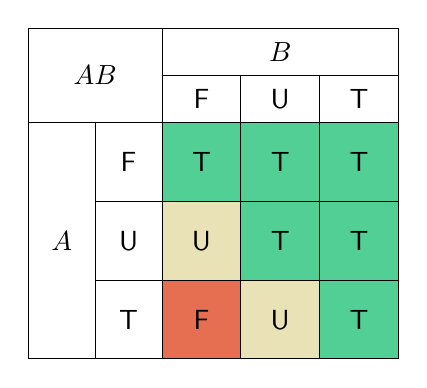
\begin{tikzpicture}[font=\sffamily,cell/.style={anchor=north west,draw,rectangle,minimum width=10mm,minimum height=10mm,outer sep=0pt},pt/.style={fill=ptgreen},pf/.style={fill=pfred},pu/.style={fill=pugrey},pl/.style={fill=plgrey,minimum width=8.5mm},pm/.style={fill=plgrey,minimum height=6mm}]
      \node[cell,pl]                    (t1) {$\mathsf{F}$};
      \node[cell,pl,minimum height=30mm,anchor=north east] at (t1.north west) (l1) {$A$};
      \node[cell,pl] at (t1.south west) (t2) {$\mathsf{U}$};
      \node[cell,pl] at (t2.south west) (t3) {$\mathsf{T}$};
      \node[cell,pm,anchor=south west] at (t1.north east) (b1) {$\mathsf{F}$};
      \node[cell,pm,anchor=south west,minimum width=30mm] at (b1.north west) (l2) {$B$};
      \node[cell,anchor=south east,minimum width=17mm,minimum height=12mm] at (b1.south west) (l3) {$A \predimp B$};
      \node[cell,pm] at (b1.north east) (b2) {$\mathsf{U}$};
      \node[cell,pm] at (b2.north east) (b3) {$\mathsf{T}$};
      \node[pt,cell] at (t1.north east) (n1) {$\mathsf{T}$};
      \node[pt,cell] at (n1.north east) (n2) {$\mathsf{T}$};
      \node[pt,cell] at (n2.north east) (n3) {$\mathsf{T}$};
      \node[pu,cell] at (n1.south west) (n4) {$\mathsf{U}$};
      \node[pt,cell] at (n4.north east) (n5) {$\mathsf{T}$};
      \node[pt,cell] at (n5.north east) (n6) {$\mathsf{T}$};
      \node[pf,cell] at (n4.south west) (n7) {$\mathsf{F}$};
      \node[pu,cell] at (n7.north east) (n8) {$\mathsf{U}$};
      \node[pt,cell] at (n8.north east) (n9) {$\mathsf{T}$};
    \end{tikzpicture}
  \end{subfigure}\hfill%
  \begin{subfigure}{0.32\linewidth}
    \centering
    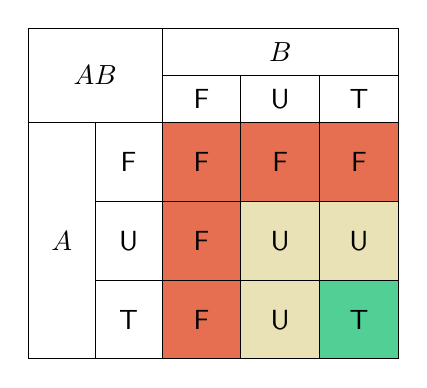
\begin{tikzpicture}[font=\sffamily,cell/.style={anchor=north west,draw,rectangle,minimum width=10mm,minimum height=10mm,outer sep=0pt},pt/.style={fill=ptgreen},pf/.style={fill=pfred},pu/.style={fill=pugrey},pl/.style={fill=plgrey,minimum width=8.5mm},pm/.style={fill=plgrey,minimum height=6mm}]
      \node[cell,pl]                    (t1) {$\mathsf{F}$};
      \node[cell,pl,minimum height=30mm,anchor=north east] at (t1.north west) (l1) {$A$};
      \node[cell,pl] at (t1.south west) (t2) {$\mathsf{U}$};
      \node[cell,pl] at (t2.south west) (t3) {$\mathsf{T}$};
      \node[cell,pm,anchor=south west] at (t1.north east) (b1) {$\mathsf{F}$};
      \node[cell,pm,anchor=south west,minimum width=30mm] at (b1.north west) (l2) {$B$};
      \node[cell,anchor=south east,minimum width=17mm,minimum height=12mm] at (b1.south west) (l3) {$A \predand B$};
      \node[cell,pm] at (b1.north east) (b2) {$\mathsf{U}$};
      \node[cell,pm] at (b2.north east) (b3) {$\mathsf{T}$};
      \node[pf,cell] at (t1.north east) (n1) {$\mathsf{F}$};
      \node[pf,cell] at (n1.north east) (n2) {$\mathsf{F}$};
      \node[pf,cell] at (n2.north east) (n3) {$\mathsf{F}$};
      \node[pf,cell] at (n1.south west) (n4) {$\mathsf{F}$};
      \node[pu,cell] at (n4.north east) (n5) {$\mathsf{U}$};
      \node[pu,cell] at (n5.north east) (n6) {$\mathsf{U}$};
      \node[pf,cell] at (n4.south west) (n7) {$\mathsf{F}$};
      \node[pu,cell] at (n7.north east) (n8) {$\mathsf{U}$};
      \node[pt,cell] at (n8.north east) (n9) {$\mathsf{T}$};
    \end{tikzpicture}
  \end{subfigure}\hfill%
  \begin{subfigure}{0.32\linewidth}
    \centering
    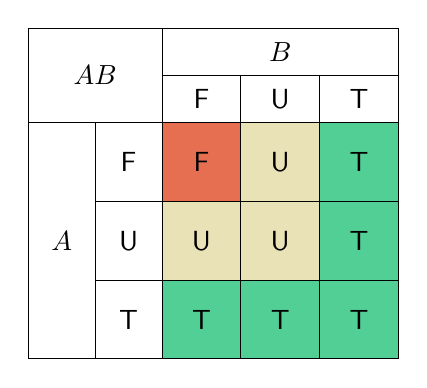
\begin{tikzpicture}[font=\sffamily,cell/.style={anchor=north west,draw,rectangle,minimum width=10mm,minimum height=10mm,outer sep=0pt},pt/.style={fill=ptgreen},pf/.style={fill=pfred},pu/.style={fill=pugrey},pl/.style={fill=plgrey,minimum width=8.5mm},pm/.style={fill=plgrey,minimum height=6mm}]
      \node[cell,pl]                    (t1) {$\mathsf{F}$};
      \node[cell,pl,minimum height=30mm,anchor=north east] at (t1.north west) (l1) {$A$};
      \node[cell,pl] at (t1.south west) (t2) {$\mathsf{U}$};
      \node[cell,pl] at (t2.south west) (t3) {$\mathsf{T}$};
      \node[cell,pm,anchor=south west] at (t1.north east) (b1) {$\mathsf{F}$};
      \node[cell,pm,anchor=south west,minimum width=30mm] at (b1.north west) (l2) {$B$};
      \node[cell,anchor=south east,minimum width=17mm,minimum height=12mm] at (b1.south west) (l3) {$A \predor B$};
      \node[cell,pm] at (b1.north east) (b2) {$\mathsf{U}$};
      \node[cell,pm] at (b2.north east) (b3) {$\mathsf{T}$};
      \node[pf,cell] at (t1.north east) (n1) {$\mathsf{F}$};
      \node[pu,cell] at (n1.north east) (n2) {$\mathsf{U}$};
      \node[pt,cell] at (n2.north east) (n3) {$\mathsf{T}$};
      \node[pu,cell] at (n1.south west) (n4) {$\mathsf{U}$};
      \node[pu,cell] at (n4.north east) (n5) {$\mathsf{U}$};
      \node[pt,cell] at (n5.north east) (n6) {$\mathsf{T}$};
      \node[pt,cell] at (n4.south west) (n7) {$\mathsf{T}$};
      \node[pt,cell] at (n7.north east) (n8) {$\mathsf{T}$};
      \node[pt,cell] at (n8.north east) (n9) {$\mathsf{T}$};
    \end{tikzpicture}
  \end{subfigure}
  \caption[Truth tables for three-valued logic operators.]{Truth tables corresponding to the three-valued logic operators, where $\mathsf{T}$, $\mathsf{U}$ and $\mathsf{F}$ are abbreviations for $\predtrue$, $\predundef$ and $\predfalse$ respectively.}%
  \label{fig:three-valued-truth-table}
\end{figure}%
%
This is a pure three-valued logic formula using \L{}ukasiewicz three-valued
logic semantics \cite{borowski70_swj}, where the truth tables for \enquote{implication}, \enquote{and} and \enquote{or} are given in \cref{fig:three-valued-truth-table}.  This
interpretation of three-valued logic is chosen because it allows for tautologies
in the logic.  In the standard interpretation of three-valued logic where
implication is defined in terms of $\predand$ and $\predor$, every expressable
formula will evaluate to $\predundef$ if all the variables are set to
$\predundef$ because $\predundef \rightarrow \predundef \equiv \predundef$.
\L{}ukasiewicz three-valued logic, on the other hand, has the following
behaviour for implication $\predundef \predimp \predundef \equiv \predtrue$, also shown in the truth table in \cref{fig:three-valued-truth-table},
meaning one can express formulas that are tautologies to show that a certain property will always hold.
As a concrete example, $(a \rightarrow a) \leftrightarrow \predtrue$ would not be provable in the more standard formulation of three-valued logic, because $a$ can always be set to $\predundef$, whereas $(a \predimp a) \equiv \predtrue$ is provable, because even if $a$ is set to $\predundef$, the formula will still evaluate to $\predtrue$.

\begin{figure}%
\begin{mathpar}
\inferrule[]{ }{\evalpred{\rs}{\predtrue}{\bvrai}}
\and
\inferrule[]{ }{\evalpred{\rs}{\predfalse}{\bfalse}}
\and
\inferrule[]{ }{\evalpred{\rs}{\predundef}{\boolundef}}
\and
\inferrule[]
          { }
          {\evalpred{\rs}{\predatompos{\varcond}}{\at{\rs}{\varcond}}}
\and
\inferrule[]
          { }
          {\evalpred{\rs}{\predatomneg{\varcond}}{1-\at{\rs}{\varcond}}}
\and
\inferrule[]
          {\evalpred{\rs}{\varpred_1}{\varbool_1} \\
           \evalpred{\rs}{\varpred_2}{\varbool_2}
          }
          {\evalpred{\rs}{\varpred_1 \predor \varpred_2}{\varbool_1 \boolor
              \varbool_2}}
\and
\inferrule[]
          {\evalpred{\rs}{\varpred_1}{\varbool_1} \\
           \evalpred{\rs}{\varpred_2}{\varbool_2}
          }
          {\evalpred{\rs}{\varpred_1 \predand \varpred_2}{\varbool_1 \booland
              \varbool_2}}
\and
\inferrule[]
          {\evalpred{\rs}{\varpred_1}{\varbool_1} \\
           \evalpred{\rs}{\varpred_2}{\varbool_2}
          }
          {\evalpred{\rs}{\varpred_1 \predimp \varpred_2}{1 \booland
              (1 - \varbool_1 + \varbool_2)}}
\end{mathpar}
\caption[Evaluation of three-valued logic predicates.]{Evaluation of three-valued logic
  predicates, where $\rs$ is a valuation from predicate variables $c$ to
  $\set{\bvrai,\bfalse,\boolundef}$.}%
\label{fig:evalpred}
\end{figure}%

The final steps of the validation are therefore to translate the three-valued
logic equation into a form that is accepted by SMTCoq.  For this, we give an interpretation of the three-valued logic in linear arithmetic, which is shown in \cref{fig:evalpred}.  Let us try to prove that the following formula always holds:
$\syniteformulanslk{c_1}{\predtrue}{\predtrue}$.  Using the linear arithmetic interpretation, this would give the following SMT formula, where all
the variables are constrained to be between $\bfalse$ and $\bvrai$, i.e.
$\forall n\ldotp \bfalse \leq c_n \leq \bvrai$.  The constraint has been left
out from the formulation below for simplicity, but would have to be added to the
actual formulation.  Finally, we check that this formula does not equal 1,
meaning if the SMT solver returns \texttt{unsat}, then the formula should always
hold.
%
\begin{equation}
  (1 \booland (1 - c_1 + 1)) \booland (1 \booland (1 - (1 - c_1) + 1)) \neq 1.
\end{equation}
%
Internally, SMTCoq uses an efficient
and compact array structure to represent the formula, which is split into three
main parts, the array for the atoms of the formula, the array for formula
components, and finally the array containing the formula itself, called the
roots.  When translated to the array representation, the above formula would be represented as follows
in SMTCoq, where we have the list of atoms $a$, which are made up of a boolean
true ($\top$) and false ($\bot$), in addition to the two atoms that are needed
to encode the formula above, namely $1$ and the variable $c_1$.  Then, the
formula is constructed as a list of formulas that either reference elements
earlier in the list or atoms, and encode the formula above.  Finally, the root
contains a reference to the formula that should be checked by the SMT solver.
%
\begin{equation}
  \begin{array}{ll}
    \text{atoms: } & a = [\top; \bot; 1; c_1]\\
    \text{formulas: } & f = [a[2]; a[3]; f[0] - f[1]; f[2] + f[0]; f[0]
                        \booland f[3];\\
                   & \qquad f[0] - f[2]; f[5] + f[0]; f[0] \booland
                     f[6]; f[4] \land f[7]; f[8] \neq f[0]]\\
    \text{roots: } & r = [f[9]].
  \end{array}
\end{equation}

The original SMT formula can then be passed to an SMT solver to check for
unsatisfiability.  This is done using veriT~\cite{bouton09}, which is well
supported by SMTCoq.  The witness, together with the array representation of the
formula are then read by the SMTCoq proof checker, which emits \enquote{yes} or
\enquote{no} depending on if checking the witness succeeded, in which case the
formula that was checked was unsatisfiable or not.  This result can be used to
check the equivalence between two predicate expressions at run time and assume
that if the check succeeds, that the predicate expressions can be assumed to be
equivalent.

\section{Summary}

We have presented the first verified implementations of general if-conversion
and hyperblock scheduling, and incorporated them into the Vericert verified HLS
tool. The practical value of this work is that it makes verified \gls{HLS}
practical by validating an industry standard scheduling algorithm. On the more
conceptual side, our work may prove useful to those implementing other
optimisation passes in a verified compiler using solver-powered validation.  For
example, this back end was also used to verify the construction of gated-SSA,
where three-valued logic validation was also needed to show that path predicates
were correct~\cite{herklotz23_msgssa}.

There are opportunities for further performance improvements by tweaking the
if\?conversion heuristics and the implementation of the scheduler. Both of these
should be relatively straightforward because neither affects the correctness
proof. Longer term, we plan to implement further optimisations in Vericert, such
as modulo scheduling~\cite{zhang13_sdc}, which would enable loops to be
pipelined.

%%% Local Variables:
%%% mode: latex
%%% TeX-master: "../thesis"
%%% TeX-engine: luatex
%%% End:
